\documentclass[draftthesis,fancy,edeposit]{uiuc_thesis_template}

\usepackage{epigraph}

\begin{document}

\title{Using Machine Learning Techniques to Estimate Lepton Backgrounds in Supersymmetry Physics Searches with the ATLAS Detector}
\author{Matt Zhang}
\department{Physics}
\schools{B.S. University of Texas at Austin, 2013}
\phdthesis
\advisor{Ben Hooberman}
\degreeyear{2019}
\committee{Professor Ben Hooberman\\Professor Mark Neubaeur\\Professor Jessie Shelton\\Professor Lance Cooper}
\maketitle

\frontmatter

\begin{abstract}
We demonstrate the use of machine learning techniques to enhance physics searches using data from the ATLAS detector at CERN. Neural nets 4ever.
\end{abstract}

\begin{dedication}
This thesis is for my friends, who almost managed to keep me sane after all these years.
\end{dedication}

\chapter*{Acknowledgments}

Thank Ben, thank CERN, thank Blue Waters? I'm not sure who else I have to thank but be sure to thank them all.

\tableofcontents
\listoftables
\listoffigures

\chapter*{List of Abbreviations and Definitions}

\begin{symbollist*}
\item[ATLAS] A Toroidal LHC ApparatuS. A detector at the LHC.
\item[LHC] Large Hadron Collider. A circular proton-proton collider operating at CERN.
\item[CERN] Conseil Européen pour la Recherche Nucléaire. A multinational high-energy physics experiment operating on the French-Swiss border.
\end{symbollist*}

\mainmatter

\part{A Brief Introduction to the Theory}
\chapter{The History of Understanding the History of Everything}

In the beginning people knew nothing. What is the universe made of? Can you turn a rock into gold? What happens if you get smaller and smaller - is there a whole different world down there? These were just a small subset of questions our early ancestors would never know the answer to, since they all died out before the development of particle physics in the $20^{th}$ century. But let's entertain ourselves by examining a few of the early mental models they had, and how the persistent desire to improve these models led to the development of modern physics.

\section{The Basic Components}

It's somewhat strange at first glance that many ancient cultures had roughly the same classic elements, but upon examination of the things commonly found in nature, we can understand where these groupings came from. Most early building materials, food, and organic compounds came out of and into the earth. These things seemed to cycle endlessly and turn easily into each other, so the element of earth or clay logically served as a catch-all building block for all such materials. Chinese philosophy further divided wood and metal into their own categories separate from earth. Next came fire and water, distinct enough from earth to warrant separate categories of their own. Together, earth, water, and fire also roughly corresponded to the common states of matter (solid, liquid, gas/plasma), so it's understandable that these mental clusterings became common in many early philosophies. The elements of air and aether were somewhat unique to Greek thought however, and were probably later transported into India and folded into the classic Buddhist elements.

In all then, we had air, water, earth, fire, and aether in Greek philosophy, corresponding to the five Platonic solids~\cite{Plato}, and according to Empedocles~\cite{Empedocles}, bound together by love and strife. In Indian philosophy we had air, water, and earth, corresponding to different categories of food~\cite{Chandogya}. This evolved with Greek influence into the five elements of early Buddhism and Hinduism, each with their own associations~\cite{friesian}. In Chinese philosophy we had metal, wood, earth, water, and fire~\cite{Tao}. When combined with air and aether, the system was further expanded to form associations with the sun, moon, and five visible planets~\cite{friesian}.

And so we see how throughout the ancient world, a complex series of inter-related, "common-sense", and entirely wrong memetic systems came to dominate early philosophy. Based on pattern recognition and concept association rather than experimental evidence, these unscientific models guided intellectual pursuits for many centuries.

<The_Sceptical_Chymist>

<chemical revolution>

<John Dalton>

<Einstein brownian motion>

<Mendeleev>

\section{Elements Are Not Elemental}

\section{A New Subatomic World}

\section{Everything Is Particles}
\chapter{The Standard Model of Physics}\label{chap:SM}

\section{The History of Understanding the History of Everything}

In the beginning people knew nothing. What is the universe made of? Can you turn a rock into gold? What happens if you get smaller and smaller - is there a whole different world down there?

\subsection{Early Beliefs}

\subsection{The Basic Components}

\subsection{Elements Are Not Elemental}

\subsection{A New Subatomic World}

\section{Everything Is Particles}

\subsection{Electrifying Discoveries}

\subsection{Smashing the Proton}

\subsection{Photographing a Ghost}

\subsection{The Particle Nobody Ordered}

\subsection{A Confusing Explosion}

\subsection{Order to the Chaos}

\subsection{The Final Piece of the Puzzle}

\section{Physics Is Not Over}

\subsection{Problems with the Standard Model}

\subsection{What Particle Physicists Do All Day}
\chapter{Supersymmetry}

\section{What Is Supersymmetry?}

\section{Theoretical Support}

\section{How to Find SUSY}

\section{Failing to Find SUSY}

\section{How Long Can This Madness Go On For?}

\part{How CERN Conducts Experiments}
\chapter{The Hardware}

\section{The Layout of CERN}

\setlength{\epigraphwidth}{3in}
\epigraph{Later for the date than the Hadron Collider}{MF Doom, Gazzillion Ear}

\section{An Anatomy of ATLAS}

\subsection{Calorimeters}

%%%%%%%%%%%%%%%%%%%%%%%%%%%%%%%%%%%%%%%%%%%%%%%%%%%%%%%%%%%

The Large Hadron Collider (LHC) is a 27-kilometer long proton-proton circular collider located underneath the border area of France and Switzerland, outside the city of Geneva. After accelerating protons to extremely high kinetic energies, the collider smashes two proton beams head-on at a center-of-mass energy of 13 TeV, converting the energy into mass and producing a spray of new particles. These collision events take place at four beam-crossing points located around the circumference of the accelerator ring, and the resulting data is captured by seven detectors. One of these detectors, ATLAS, is the focus of this study.

The ATLAS detector (Figure~\ref{ATLAS}), built around one of the LHC beam crossing points, acts as a eight-story-tall recording device for measuring and digitizing the results of collisions. The detector contains multiple types of detection technology, each specialized to perform a specific type of measurement \cite{ATLAS_website}. The first major component of ATLAS is the inner detector. Composed of silicon pixel and strip detectors and transition radiation trackers, this portion of the detector is used to reconstruct the flight paths and momentums of charged particles. After this we have the electron calorimeter (ECAL), which captures and records the energies of electrons and photons through EM interactions. The hadronic calorimeter (HCAL) is after that, and being composed of heavy elements, it forces hadronic particles to deposit their energies through strong interactions. Finally, the detector is ringed by muon spectrometers, which detect the penetrating muons that pass unstopped through the rest of the detector. Neutrinos pass through ATLAS undetected, and their effects are seen in missing transverse momentum when the transverse momentums of all other decay products in the reaction are summed vectorially. These particle interactions are summed up in Figure~\ref{ATLAS}. Based on the hits recorded in a single collision, algorithms then reconstruct tracks, determine what particles were involved in the event, and figure out what happened in their brief lifetimes.
%A typical reconstructed event is shown in Figure~\ref{Higgs_2e2mu}. Here we see a Higgs boson decaying into two electrons and two muons. The muons, shown in red, pass through the detector, while the electrons shown in green deposit their energies in the ECAL. In this event, based on the energies of decay products, the original Higgs has been measured to have a mass of 122.6 GeV.

\begin{figure}[t]
    \centering
    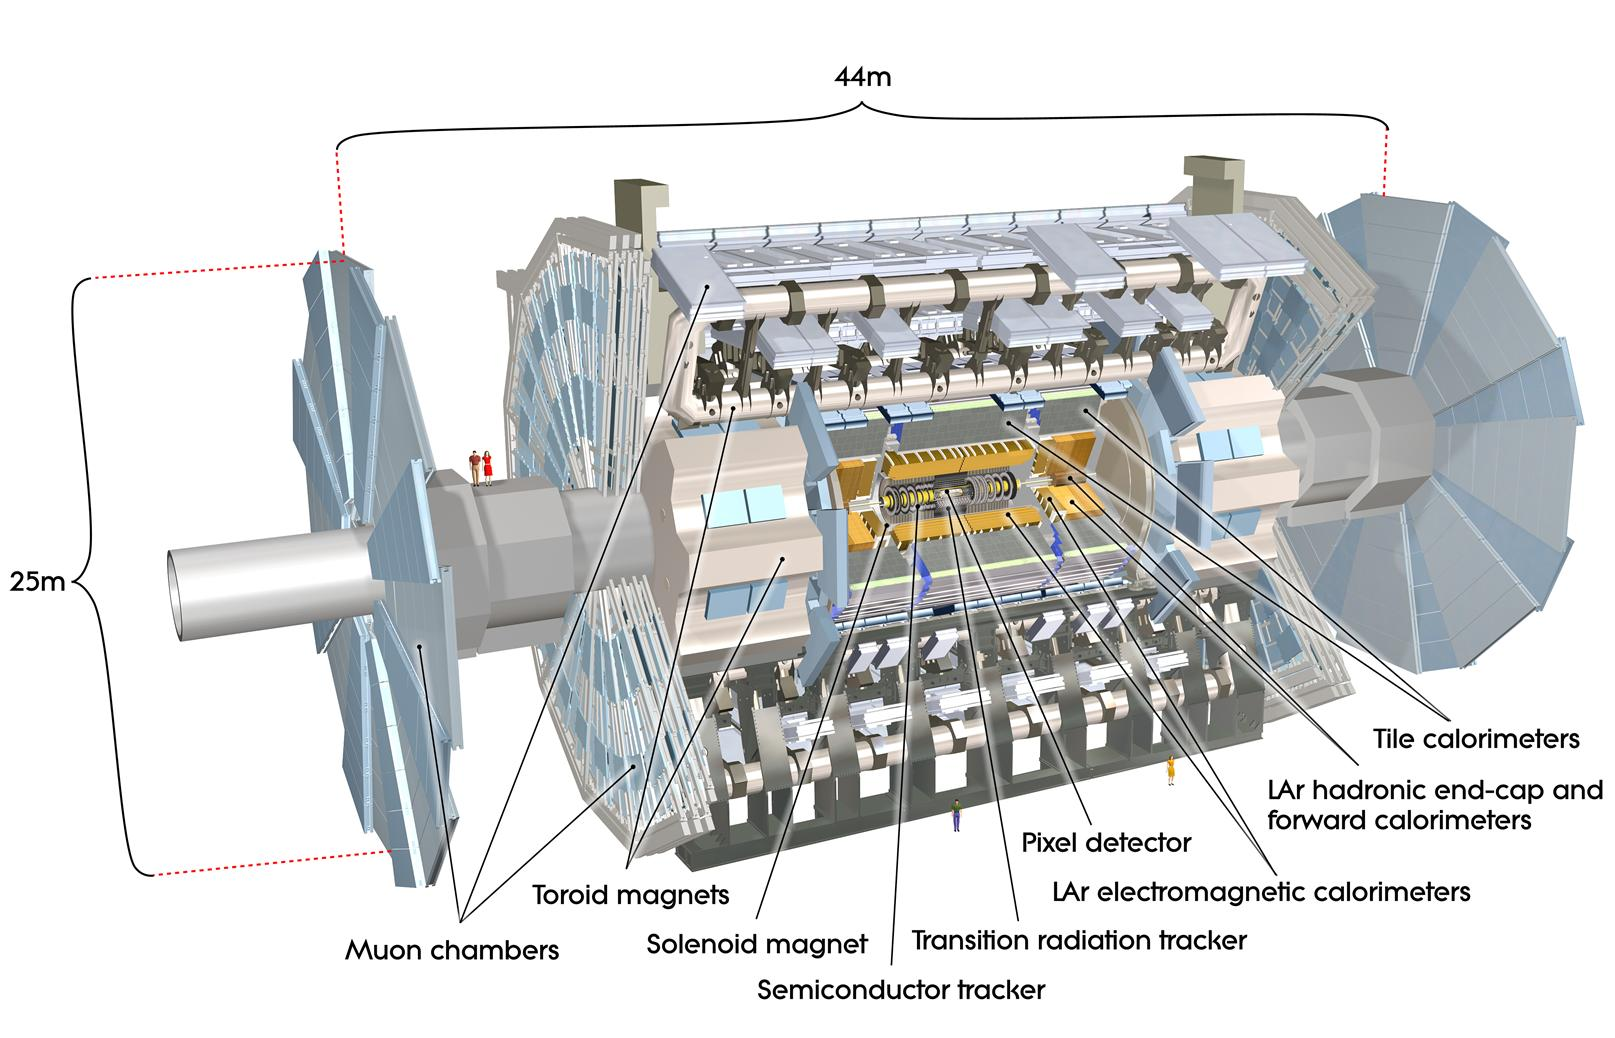
\includegraphics[width=0.49\linewidth]{images/ATLAS.png}
    \includegraphics[width=0.41\linewidth]{images/ATLASinteractions.jpg}
    \caption{(left) A labeled diagram of the ATLAS detector. (right) Interactions of different types of particles in ATLAS.}
    \label{ATLAS}
\end{figure}

%\begin{figure}[t]
%    \centering
%    \includegraphics[width=0.5\linewidth]{images/Higgs_2e2mu.png}
%    \caption{A typical reconstructed event display, showing a Higgs boson decaying into two electrons and two muons \cite{Higgs_2e2mu}.}
%    \label{Higgs_2e2mu}
%\end{figure}

\subsection*{Upgrades}

The LHC currently produces about 40 collisions per beam-crossing at 13 TeV center-of-mass energy, but with the proposed high-luminosity LHC (HL-LHC) upgrade there are plans to increase these numbers to 140 collisions per beam-crossing at 14 TeV by 2026, amounting to a total of 250 $fb^{-1}$ of data per year, with ultimate plans to increase to 200 collisions per beam-crossing. During the HL-LHC upgrade, ATLAS similarly plans to upgrade its detection capabilities via the ATLAS Phase-II upgrade, focusing on items such as replacing the inner detector with an all-silicon-based inner tracker (ITk), improving data acquisition, and increasing the granularity of calorimeters \cite{ATLAS_phaseII}. The higher data rates and improved calorimeters provide an incentive to develop and implement the machine-vision based particle identification systems described later in this paper. In the interest of improving upcoming SUSY searches, I have aided in the development of several components in the ATLAS detector. Though they will not be the focus of this paper, as they mostly impact future analyses, I would like to mention them in passing.

First, I worked on investigating methods for improving vertex reconstruction for use in future high-pileup environments, as part of the vertex reconstruction group at ATLAS. The approach we used was based on dividing physical space into a grid of three-dimensional pixels, and using reconstructed tracks to "fill in" those pixels and generate a 3D image. The resulting image was then Fourier transformed, filtered to remove high frequencies, reverse Fourier transformed, and collapsed along the beam axis, resulting in a 1D function where the peaks corresponded to potential vertex locations (vertex "seeds"). Tracks were then associated with their nearest seeds, and from each cluster of tracks we fit a final vertex. I performed performance comparisons between the new and old vertexing methods, and did studies based on tuning parameters of the new method. Some of these results were shown in my presentation at the 2015 ATLAS CP Tracking Workshop \cite{vertex}. I also performed studies on using machine-learning methods to better associate tracks with vertex seeds, and to recognize and recombine "split" vertices, though these methods did not show significant improvements over baseline during my time with the project.

I also performed some work on upgrades to the ITk for the ATLAS Phase-II upgrade. Recently I spent a year at Argonne under the guidance of Dr. Jessica Metcalfe working on manufacturing methods for mass production of silicon pixel detectors in preparation for the upgrade. During that time I worked on setting up a manufacturing lab and various electronic test environments, on assembling pixel modules using various mechanical epoxy-based techniques, on designing adapter boards for readout electronics, and on performing tests on assembled modules. I also participated in a three-month testbeam at Fermilab with the University of Geneva, during which we gathered and analyzed data from a proposed HVCMOS pixel detector. The idea behind this detector was that due to advances in silicon sensor manufacturing, we could build readout circuitry directly into the detector, removing the need for an external readout chip. This resulted in less detector material, and also reduced manufacturing cost. I presented results from this testbeam at DPF 2017 \cite{DPF}, and this analysis, combined with additional data taken by the University of Geneva at the SPS in CERN, will be presented in an upcoming paper on the new detector.

Furthermore, I have contributed some work to the fast tracker (FTk) upgrade for ATLAS \cite{FTk}. The FTk is an FPGA-based method for performing online track reconstruction, for use in the inner detector. I worked on the extrapolator board with Professor Mark Neubaeur's team. The extrapolator is responsible for reconstructing 12-layer tracks (for the 12 layers of the inner detector) using preliminary 8-layer tracks and a collection of hits from the other 4 layers. I developed a new memory storage mechanism for organizing and retrieving hits, and have recently completed a rewrite of the extrapolation code. We are currently working to ensure uninterrupted data flow, and are attempting to optimize our firmware to run at 200 MHz.
\chapter{The Software}

\section{Event Reconstruction}

\section{Data Storage and Processing}

\section{Monte Carlo}
\chapter{How to Do a Search}

\section{Model Selection}

\section{Region Selection}

\subsection{Background Identification}\label{sec:background}

\subsection{Finding the Best Cuts}

\section{Background Estimation}

\section{Interpreting Results}

\subsection{Unblinding and Comparison}

\subsection{How to Read Result Plots}

\part{Machine Learning}
\chapter{Machine Learning}

\section{Building a Thinking Machine}

\subsection{Conscious Decision Making As an Algorithm}

\subsection{Fumbling Towards a Solution}

\subsection{Tools for Fumbling Faster}

\section{An Analysis Pipeline}

\section{Modelling a Brain}

\subsection{Neural Layers}

\subsection{Classification and Regression}

\section{Neural Architectures}

\subsection{Convolutional Nets}

\subsection{Generative Adversarial Nets}

\subsection{Recurrent Neural Nets}\label{sec:RNN}
\chapter{Neural Architectures}

\section{Convolutional Nets}

\section{Generative Adversarial Nets}

\section{Recurrent Neural Nets}\label{sec:RNN}

%%%%%%%%%%%%%%%%%%%%%%%%%%%%%%%%%%%%%%%%%%%%%%%%%%%%%%%%%%%

Machine learning is an area of computer science in which we attempt to create intelligent systems that are able to make complex, human-level decisions. It has seen use in recent years in areas as diverse as self-driving cars, language processing, and automatic crop harvesting. In recent years, many machine learning techniques have started being applied to the realm of high-energy physics. Due to very high volumes of data production, especially for planned next-gen colliders such as the HL-LHC, and due the complexity involved in reconstructing each collision event, machine learning has been applied to applications such as track reconstruction, vertex-finding, and jet identification, and was used in the Higgs discovery. The field is extremely broad with many applications, so I will only attempt to describe a few basic ideas here.

Boiled down to its fundamentals, the goal of a machine learning process is  to take a set of input data, and to generate the optimal outputs. For instance, a facial recognition system may take as its inputs a set of pixels originating from a camera or video feed, and output a pointer to a name in a database of people. A translation program may take a string of characters in one language as text input and output another string in a different language. A drone with obstacle avoidance may take input from visual systems and from mounted sensors, and output instructions to its various motors. Even an organic entity takes chemical, physical, and internal inputs from its environment, and outputs chemical and electrical signals to its muscles and organs. There are two major classifications of machine-learning algorithms. One type is supervised, where a system is fed a series of training examples, and is told explicitly what type of output the system should be attempting to obtain for each example. This is the case for an image-classification algorithm, which may be fed many different input images, along with labels for each image. The other major type of machine learning algorithm is unsupervised. In this case, the algorithm is still fed input data, but is not told what the output should be. This is generally the case for clustering algorithms, such as those used for data compression and error/outlier detection.

To build a particle recognition system, we will eventually require unsupervised learning in order to implement systems that recognize and zoom in on energy clusters. However, in the interest of conciseness, I will focus only on supervised algorithms here. As its name suggests, the field of machine learning is generally focused on how to get an algorithm to "learn" from input data. In a supervised learning example, the algorithm takes the form of a complicated expression with many tunable parameters. This expression may be in the form of a series of matrix operations, or as a chain of cut-based classifiers, or in general any other form of an input-output system with tunable components. This algorithm begins with some initialized parameters, and is fed a chunk of input data (which may be composed of one or several input examples). The algorithm then spits out its outputs, which are compared to the correct outputs. The accuracy of the response is then quantified using a "loss function", which in practice is often either the L2 distance, the logistic loss function, or the cross entropy loss. I will now talk about two very common algorithms, the boosted decision tree (BDT) and neural net (NN).

\section{BDT}

Simply speaking, a decision tree is simply a series of branching paths based on input data, which one can follow to reach a conclusion. An example of a very simple decision tree is shown in Figure~\ref{decision_tree}. Decision trees are similar to how objects and signal regions are selected in a traditional high-energy-physics analysis. For example, one may ask whether an event has more than, less than, or equal to three leptons. If the event has exactly three leptons, one may ask whether the top two leptons have dilepton mass within a certain range, etc. Based on these decisions, an experimenter can decide what signal region an event belongs in. As another example, imagine that we are trying to determine what kind of particle we have seen in an event. We could ask whether the particle left a track in the inner detector, whether the amount of energy it deposited in the calorimeter is in a certain range, etc. Given a random ordered set of input variables, an optimal decision tree can be calculated for decisions made in that specific order.

A boosted decision tree is created by combining many different decision trees together \cite{BDT}. Any given decision tree can be very weak, containing only a small number of branches and a small maximum depth. However, by taking the weighted results of many decision trees together, we can get a more accurate result than can be achieved by any single tree. For the sake of space, the AdaBoost BDT training algorithm will not be discussed here.

\begin{figure}[t]
    \centering
    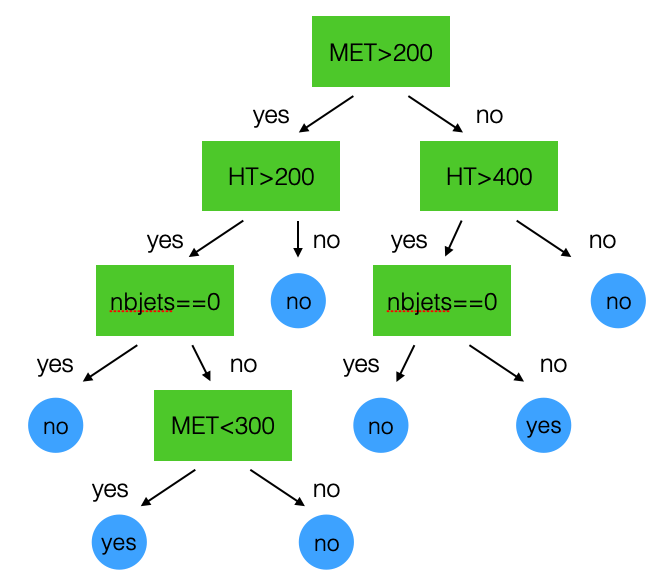
\includegraphics[width=0.5\linewidth]{images/decision_tree.png}
    \caption{An example of a decision tree that a child may use to classify a household pet.}
    \label{decision_tree}
\end{figure}

\section{Neural Net}

A neural net is a machine learning architecture based on the physical structure of neurons in the human brain \cite{neural_net}. The basic unit of a neural net is a neuron, which has a numerical value, one or more inputs, and one or more outputs. These neurons are connected together so that the output of one neuron becomes the input of one or more other neurons. Here we will only consider simple feed-forward neural nets, where all the inputs to a neuron come from neurons closer to the beginning of the net, and all the outputs of that neuron go to neurons nearer the end of the net. That is, there are no "loops", and there are no connections between neurons at the same depth. The input values for an event form the first layer of neurons, and the output is derived from the last layer. Each link between neurons is associated with a "weight", or multiplicative constant. Each neuron is also associated with a "bias", or an additive constant. Letting $y_i$ be the value of the $i^{th}$ neuron, $w_{i,j}$ be the value of the weight between neurons $i$ and $j$, and $b_i$ be the bias associated with neuron $i$, we see that the value of a neuron is equal to $y_j = \sum{w_{i,j}y_i} + b_j$. Each neuron is also typically followed by a nonlinear "activation" function, so that the result of the entire net is not simply equivalent to a single matrix operation on the input. We see then that for a given set of weights and biases, we can calculate the output value for a net given any inputs.

In order to train a neural net, we use "back-propagation", meaning that for each event (or set of events) we perform gradient descent on each weight and bias in order to minimize the resulting loss function. Over the course of many events, the net can fall into a state where it produces the correct outputs with high accuracy. In this way, the neural net training is simply a form of function optimization. Many important topics, such as how to weight initialization, methods of gradient descent, net architectures, etc. will not be discussed in this paper.

\begin{figure}[t]
    \centering
    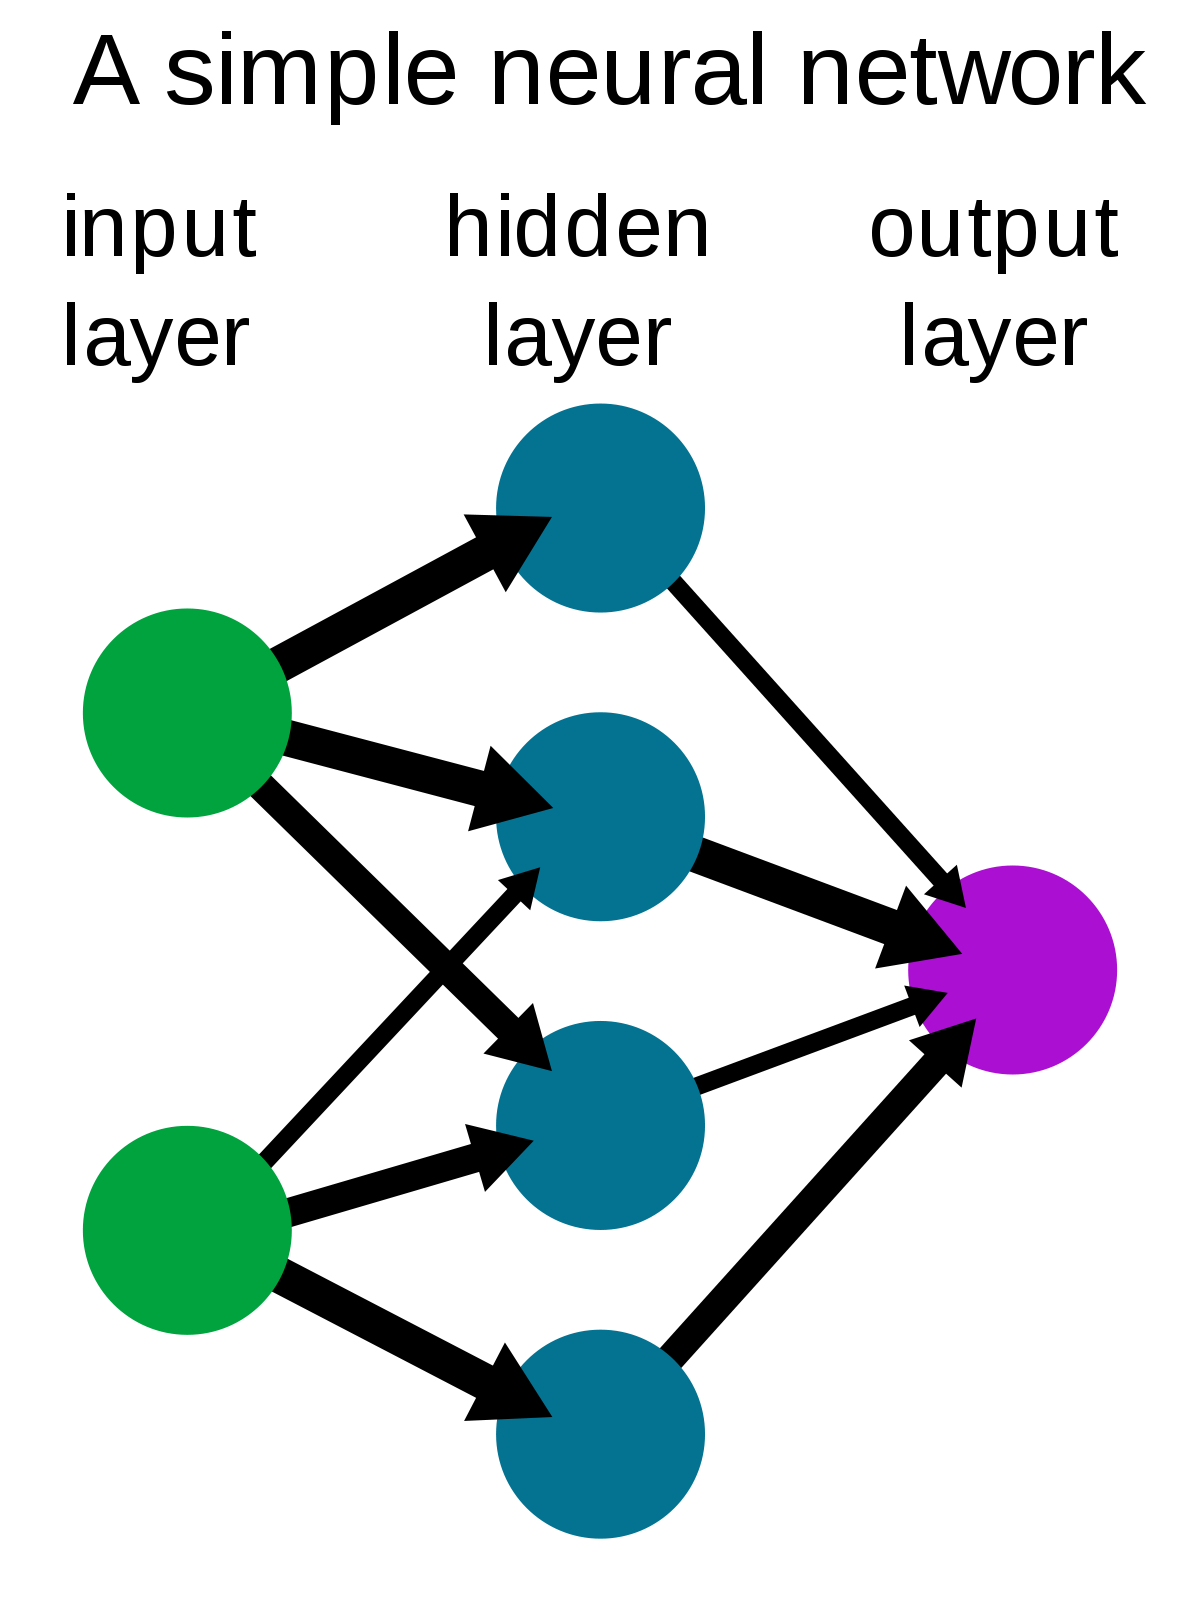
\includegraphics[width=0.5\linewidth]{images/neural_net.png}
    \caption{A diagram showing a typical densely-connected neural net.}
    \label{neural_net}
\end{figure}

\part{Particle Identification and Generation Using Calorimeter Information}
\chapter{Particle Identification and Generation Using Calorimeter Information}

\subsection{The Problem}

The next generation of detectors currently under development often feature an increase in granularity of the electromagnetic and hadronic calorimeters. This is true of the ATLAS Phase-II upgrade, and also of the highly granular CALICE sampling calorimeter proposed for the ILC, which was used for the initial studies presented in this section. These improved detector designs provide an excellent opportunity for applying machine learning algorithms for identifying particles and measuring their energies.

Our purpose in this experiment is to create a neural-net classifier using calorimeter data, which can demonstrably perform better on object identification than traditional feature-based analysis techniques can. Specifically, we have chosen to build two classifiers - one to distinguish between electrons and charged pions, and one for photons and neutral pions. In order to create a more challenging classification task, we have chosen only pion events which are likely to be confused with either electrons or photons. For charged pions, this meant taking events where the total energy deposited in the ECAL was at least 40 times greater than the energy deposited in HCAL. For neutral pions, this meant taking events where pions decayed into two photons with an opening angle of less than 0.01 radians.

The study is based on pseudo-data simulated with GEANT4 in the proposed Linear Collider Detector (LCD) for the CLIC accelerator~\cite{Lebrun}. Though we intend to extend our studies to the ATLAS detector for use in Higgsino searches, the complicated non-uniform accordion-shaped calorimeters in ATLAS add some difficulties to the task. In contrast, the LCD has uniform calorimeter cell sizes, which makes it a good starting point. The calorimeter in this detector consists of a regular grid of 3D cells with cell sizes of 5.1 mm$^3$ and an inner calorimeter radius of 1.5 m. In this dataset, individual electron, photon, charged pion, and neutral pion particles are shot orthogonally into the calorimeter surface. The particle energy is set to a fixed value of 60 GeV. For each event, a 25x25x25 cell slice of the electromagnetic calorimeter (ECAL) and the corresponding 5x5x60 cell slice of the hadronic calorimeter (HCAL) are stored as two 3D arrays of deposited energy in each cell.

We use BDT's as a proxy for traditional feature-based analysis on calorimeter data. This provides a baseline against which to compare the results of neural net performance. All features used in the BDT are calculated using traditional methods, where the complete list of features we use is as follows: total energy deposited in ECAL, total number of hits registered in ECAL, the ratio of energy deposited in ECAL first layer over energy deposited in second layer, the ratio of energy deposited in ECAL first layer over all ECAL energy, 2nd through 6th moments in the x, y, and z dimensions for ECAL energy deposits, all equivalent features for HCAL, ratio of HCAL to ECAL energy, and ratio of number of hits in HCAL to ECAL. We also examined the effect of several n-subjettiness measures, mostly to help distinguish between photons and neutral pions. Specifically, by measuring how well energy depositions were described as belonging to either one, two, or three jets, we hoped to distinguish between single photons and pions which had decayed into two photons. However, n-subjettiness was computationally expensive to calculate and did not result in much classification improvement, so its usage was dropped.

Initial studies on different net architectures showed no significant differences in performance between convolutional neural nets (CNN's) and simply-connected dense neural nets (DNN's). Therefore, we chose to focus only on DNN's, due to the smaller number of hyperparameters we would have to scan over. In the nets we trained, the ECAL and HCAL inputs were separately flattened and fed into two cell-based DNN's with identical architectures, and the outputs were merged before applying a softmax layer and computing categorical cross-entropy loss. We used two different types of nets - one based on raw cell energy inputs, and one based on the same input features that we had calculated for the BDT. This was to investigate whether differences in performance between the BDT and DNN could be attributable simply to a difference in architecture, without any actual additional information processing. Because neural nets are sensitive to the scale of input data, for the feature-based neural net we first normalized each feature by calculating the z-score for each event (i.e. $\frac{x-\bar{x}}{std(x)}$).

Each two-object classification dataset was divided into 400,000 training and 100,000 test events. After performing hyperparameter scans on Blue Waters, we decided on a DNN architecture consisting of 4 hidden layers with 256 neurons each, ReLU activation, and dropout of 0.5, trained with Adam optimization with a learning rate of 0.001. A BDT hyperparameter scan yielded best performance with 400 estimators, maximum depth of 5, and learning rate of 0.5. In our studies, we found that the most powerful feature-based discriminators are the second $x$ and $y$ moments, which measure the lateral shower width. Performance curves for the BDT's and DNN's are shown in Figure~\ref{ROCs}, and performance values are shown in Table~\ref{AUCs}.

\begin{figure}[!t]
    \centering
    \includegraphics[width=0.33\linewidth]{images/photon_pi0.pdf}
    \includegraphics[width=0.33\linewidth]{images/electron_chpi.pdf}
    \caption{Signal vs. background efficiency ROC curves for the (left) $\gamma$ vs. $\pi^0$ and (right) $e$ vs. $\pi$ classifier. The red dots mark the chosen BDT working point.}
    \label{ROCs}
\end{figure}

\begin{table}[!ht]
    \centering
    \begin{tabular}[!t]{l|cccc|cccc}
        \hline
        & \multicolumn{4}{c}{\textbf{$\gamma$ vs. $\pi^0$}} & \multicolumn{4}{c}{\textbf{$e$ vs. $\pi$}}\\
        \hline
        \textbf{Model} & \textbf{acc.} &  \textbf{AUC} & \textbf{$\Delta \epsilon_{\mathrm{sig}}$} & \textbf{$\Delta R_{\mathrm{bkg}}$} & \textbf{acc.} &  \textbf{AUC} & \textbf{$\Delta \epsilon_{\mathrm{sig}}$} & \textbf{$\Delta R_{\mathrm{bkg}}$} \\
        \hline
        \centering
        BDT & 83.1\% & 89.8\% & - & - & 93.8\% & 98.0\% & - & - \\
        DNN (features) & 82.8\% & 90.2\% & 0.9\% & 0.95 & 93.6\% & 98.0\% & -0.1\% & 0.95 \\
        DNN (cells) & 87.2\% & 93.5\% & 9.4\% & 1.63 & 99.4\% & 99.9\% & 4.9\% & 151 \\
        \hline
        \hline
    \end{tabular}
    \vspace{5pt}
    \caption{Performance parameters for BDT and DNN classifiers.} 
    \label{AUCs}
\end{table}

The areas under curve (AUC) and accuracies (acc.) for the cell-based DNNs are significantly better than for the feature-based DNNs and BDTs (which both have similar performance). This demonstrates that the DNN is able to extract additional information from the calorimeter data which is not captured via traditional measures. Choosing the working point on the BDT ROC curve indicated in Figure~\ref{ROCs}, we obtain the following improvement metrics for the cell-based DNN. For the $\gamma$ vs. $\pi^0$ ($e$ vs. $\pi^\pm$) classifier, the cell-based DNN may be used to either increase the signal efficiency by $\Delta \epsilon_{\mathrm{sig}} = \epsilon_{\mathrm{sig}}^{\mathrm{DNN}} - \epsilon_{\mathrm{sig}}^{\mathrm{BDT}}=9.4$\% (4.9\%) for fixed background efficiency, or decrease the background efficiency by a factor $\Delta R_{\mathrm{bkg}} = \epsilon_{\mathrm{bkg}}^{\mathrm{BDT}} / \epsilon_{\mathrm{bkg}}^{\mathrm{DNN}}= 1.6$ (151) for fixed signal efficiency.

\section{Overview}

In high energy physics (HEP) experiments, detectors act as imaging devices, allowing physicists to take snapshots of decay products from particle collision "events". Calorimeters are key components of such detectors. When a high-energy primary particle travels through dense calorimeter material, it deposits its energy and produces a shower of secondary particles. Detector "cells" within the calorimeter then capture these energy depositions, forming a set of voxelized images which are characteristic of the type and energy of the primary particle. %Examples of these images can be seen in Appendix~\ref{app:samples}.

The starting point of any physics analysis is the identification of the types of particles produced in each collision and the measurement of the momentum carried by each of these particles. These tasks have traditionally used manually-designed algorithms, producing measurements of physical features such as shower width and rate of energy loss for particles traversing calorimeter layers.
%In order to discover new physics or to study interesting phenomena, physicists must apply reconstruction algorithms to identify and estimate the energies of all particles produced in each event.
In the last few years, researchers have started realizing that machine learning (ML) techniques are well suited for such tasks, 
%and have recently seen application, 
e.g. using boosted decision trees (BDTs) on calculated features for doing particle classification. Indeed, ML has long been applied to various other tasks in HEP~\cite{Denby:1987rk,Peterson:1988gs,Abreu:1992jp}, including the 2012 discovery of the Higgs boson~\cite{HiggsATLAS,HiggsCMS} at the ATLAS~\cite{Aad:2008zzm} and CMS~\cite{Chatrchyan:2008aa} experiments at the Large Hadron Collider (LHC). 

In the next decade, the planned High Luminosity Large Hadron Collider (HL-LHC) upgrade~\cite{Apollinari:2284929} will enhance
the experimental sensitivity to rare phenomena by increasing the number of collected proton-proton collisions by a factor of ten. In addition, many next-generation detector components, such as the sampling calorimeters proposed for the ILC~\cite{ILC}, CLIC~\cite{CLIC}, and CMS~\cite{CMSCollaboration:2015zni} detectors, will improve physicists' ability to identify and measure particles by using much finer 3D arrays of voxels. These and future accelerator upgrades will lead to higher data volumes and pose a variety of technological and computational challenges in tasks, such as real-time particle reconstruction.

In addition to actual collision data, physics analyses typically require extremely detailed and precise simulations of detector data, generated using software packages such as GEANT4\cite{GEANT4}. These simulations are used to develop and test analysis techniques. They rely on calculations of the micro-physics governing the interaction of particles with matter, and are generally very CPU intensive. In some cases, such as the ATLAS experiment, simulation currently requires roughly half of the experiment's computing resources\cite{GEANT_usage}. This fraction is expected to increase significantly for the HL-LHC. These challenges require novel computational and algorithmic techniques, which has prompted recent efforts in HEP to apply modern ML to calorimetry~\cite{ML1,ML2,ML3,ML4}.

With this work, we aim to demonstrate the applicability of neural-network based approaches to reconstruction and simulation tasks, looking at a real use case. To do this, we use fully simulated calorimeter data for a typical collider detector to train two models: (i) a network for end-to-end particle reconstruction, receiving as input a particle shower and acting both as a particle identification algorithm and as a regression algorithm for the particle's energy; (ii) a generative adversarial network (GAN)~\cite{Goodfellow} for simulating particle showers, designed to return calorimeter-cell voxelized images like those generated by GEANT4.
Both models aim to preserve the accuracy of more traditional approaches while drastically reducing the required computing resources and time, thanks partly to a built-in portability to heterogeneous CPU+GPU computing environments.

%This paper aims to demonstrate the improvement in performance for calorimetric classification and regression tasks gained from applying various neural network architectures to calorimeter cell-level energy deposition data when compared to previously investigated ML techniques, such as boosted decision trees (BDTs) and neural networks with calculated features as inputs. We train separate networks to discriminate electrons ($e$) from charged pions ($\pi^\pm$) and to discriminate photons ($\gamma$) from neutral pions ($\pi^0$), as well as to estimate their energies and incident angles. We observe significant improvement when using neural networks with cell-level inputs, as opposed to using boosted decision trees (BDTs) or networks with high-level features. We also demonstrate an application of generative adversarial networks (GANs)~\cite{Goodfellow} for simulating particle showers, which would be computationally intensive using traditional techniques.

This paper is a legacy document summarizing two years of work. It builds upon initial simulation, classification, and regression results which we presented at the 2017 Workshop on Deep Learning for Physical Sciences at the NeurIPS conference. Those results were derived using simplified problem formulations~\cite{Mau2017}.  For instance, we only used particles of a single fixed energy for classification, and had only considered showers produced by particles traveling perpendicularly to the calorimeter surface. The results presented in this paper deal with a more realistic use case and supersede the results in Ref.~\cite{Mau2017}. 

For the studies presented in this paper, we used two computing clusters: at the University of Texas at Arlington (UTA), and at the Blue Waters supercomputing network, located at the University of Illinois at Urbana Champaign (UIUC). The UTA cluster has 10 NVIDIA GTX Titan GPUs with 6 GB of memory each. Blue Waters uses NVDIA Kepler GPUs, also with 6 GB of memory each. 

GAN models were implemented and trained using Keras~\cite{keras} and  Tensorflow~\cite{tensorflow2015-whitepaper}. Reconstruction models were implemented and trained using PyTorch~\cite{PyTorch}. The sample generation and training frameworks were both written in Python, with the sample generation codebase at \url{https://github.com/UTA-HEP-Computing/CaloSampleGeneration} and the TriForce reconstruction training framework at \url{https://github.com/BucketOfFish/Triforce_CaloML}.

This document is structured as follows: In Section~\ref{sec:data}, we describe how we created and prepared the data used in these studies. Section~\ref{sec:problems} introduces the two physics problems, particle simulation and reconstruction. Sections~\ref{sec:GAN}~and~\ref{sec:reco} describe the corresponding models, how they were trained, and the performances they reached. In particular, Section~\ref{sec:reco} compares our results to those of more traditional approaches, and also extends those comparisons to simulated performances on detector geometries similar to those of the ATLAS and CMS calorimeters. Conclusions are given in Section~\ref{sec:conclusion}.

\section{Data Preparation}

\section{Dataset}\label{sec:data}

This study is based on simulated data produced with GEANT4~\cite{GEANT4}, using the geometric layout of the proposed Linear Collider Detector (LCD) for the CLIC accelerator~\cite{Lebrun:2012hj}. We limit the study to the central region (barrel) of the LCD detector, where the electromagnetic calorimeter (ECAL) consists of a cylinder with inner radius of 1.5 m, structured as a set of 25 silicon sensor planes, segmented in $5.1~\times~5.1$ mm$^2$ square cells, alternated with tungsten absorber planes. In the barrel region, the hadronic calorimeter (HCAL) sits behind the ECAL, at an inner radius of 1.7 m. The HCAL 
consists of 60 layers of polystyrene scintillators, segmented in cells with  $3~\times~3$ cm$^2$ area and alternated with layers of steel absorbers. 

The event simulation considers the full detector layout, including the material in front of the calorimeter and the effect of the solenoidal magnetic field. From the full data we take slices centered around the barycenter of each ECAL energy deposit and we represent the ECAL and HCAL slices as 3D arrays of energy deposits in the cells. 

We consider four kinds of particles (electrons $e$, photons $\gamma$, charged pions $\pi$, and neutral pions $\pi^0$) with energies uniformly distributed between 10 and 510 GeV, and with incident angles uniformly distributed between a polar angle $\theta$ between 1.047 and 2.094 radians with respect to the beam direction.

We get the barycenter of a shower by taking the 2D projection of its energy deposit on the ECAL inner surface. Then, knowing the point of origin of the incoming particle, we use the barycenter to estimate the particle's polar and azimuthal angles $\theta$ and $\phi$. The estimated pseudorapidity $\eta$ is then computed as $\eta=-\log[\tan\frac{\theta}{2}]$. Each single-shower event is prepared by taking a slice of the ECAL in a window around the shower barycenter, as well as the corresponding HCAL slice behind. Depending on the task (generation or reconstruction), we take:
\begin{itemize}
  \item {\bf GEN dataset}: A $51 \times 51 \times 25$ cell window in the
    ECAL, for electrons in the energy range $100-200$ GeV. Used in the shower generation task.
  \item {\bf REC dataset}: A $25 \times
    25 \times 25$ cell slice of the electromagnetic calorimeter (ECAL)
    and a corresponding $11 \times 11 \times 60$ cell slice of the
    hadronic calorimeter (HCAL), for $e,~\gamma,~\pi,$~or~$\pi^0$ in the energy range $10-510$ GeV and with $\eta$ from $-0.524-0.524$. Used in the particle reconstruction task.
\end{itemize}

%%%%%%%%%%%%%%%%

Examples of an electron shower and a charged-pion shower can be seen in Figure~\ref{fig:sample}. The incoming particles enter from the top ($z=0$), at the center of the $(x,y)$ transverse plane ($x=y=25)$. The electron event has left more hits in both the ECAL and HCAL. We can also see the presence of two subtracks in the neutral pion event. % These features are characteristic of events from these two classes.

The window size for the GEN dataset has been defined in order to contain as much of the shower information as practically possible.  
Motivated by the need of reducing the memory footprint for some of the models, we used a smaller window size for the REC dataset. When training classification models on these data, a negligible accuracy increase was observed when moving to larger windows, as described in Appendix~\ref{app:window_size}.

\begin{figure*}[htbp]
\centering
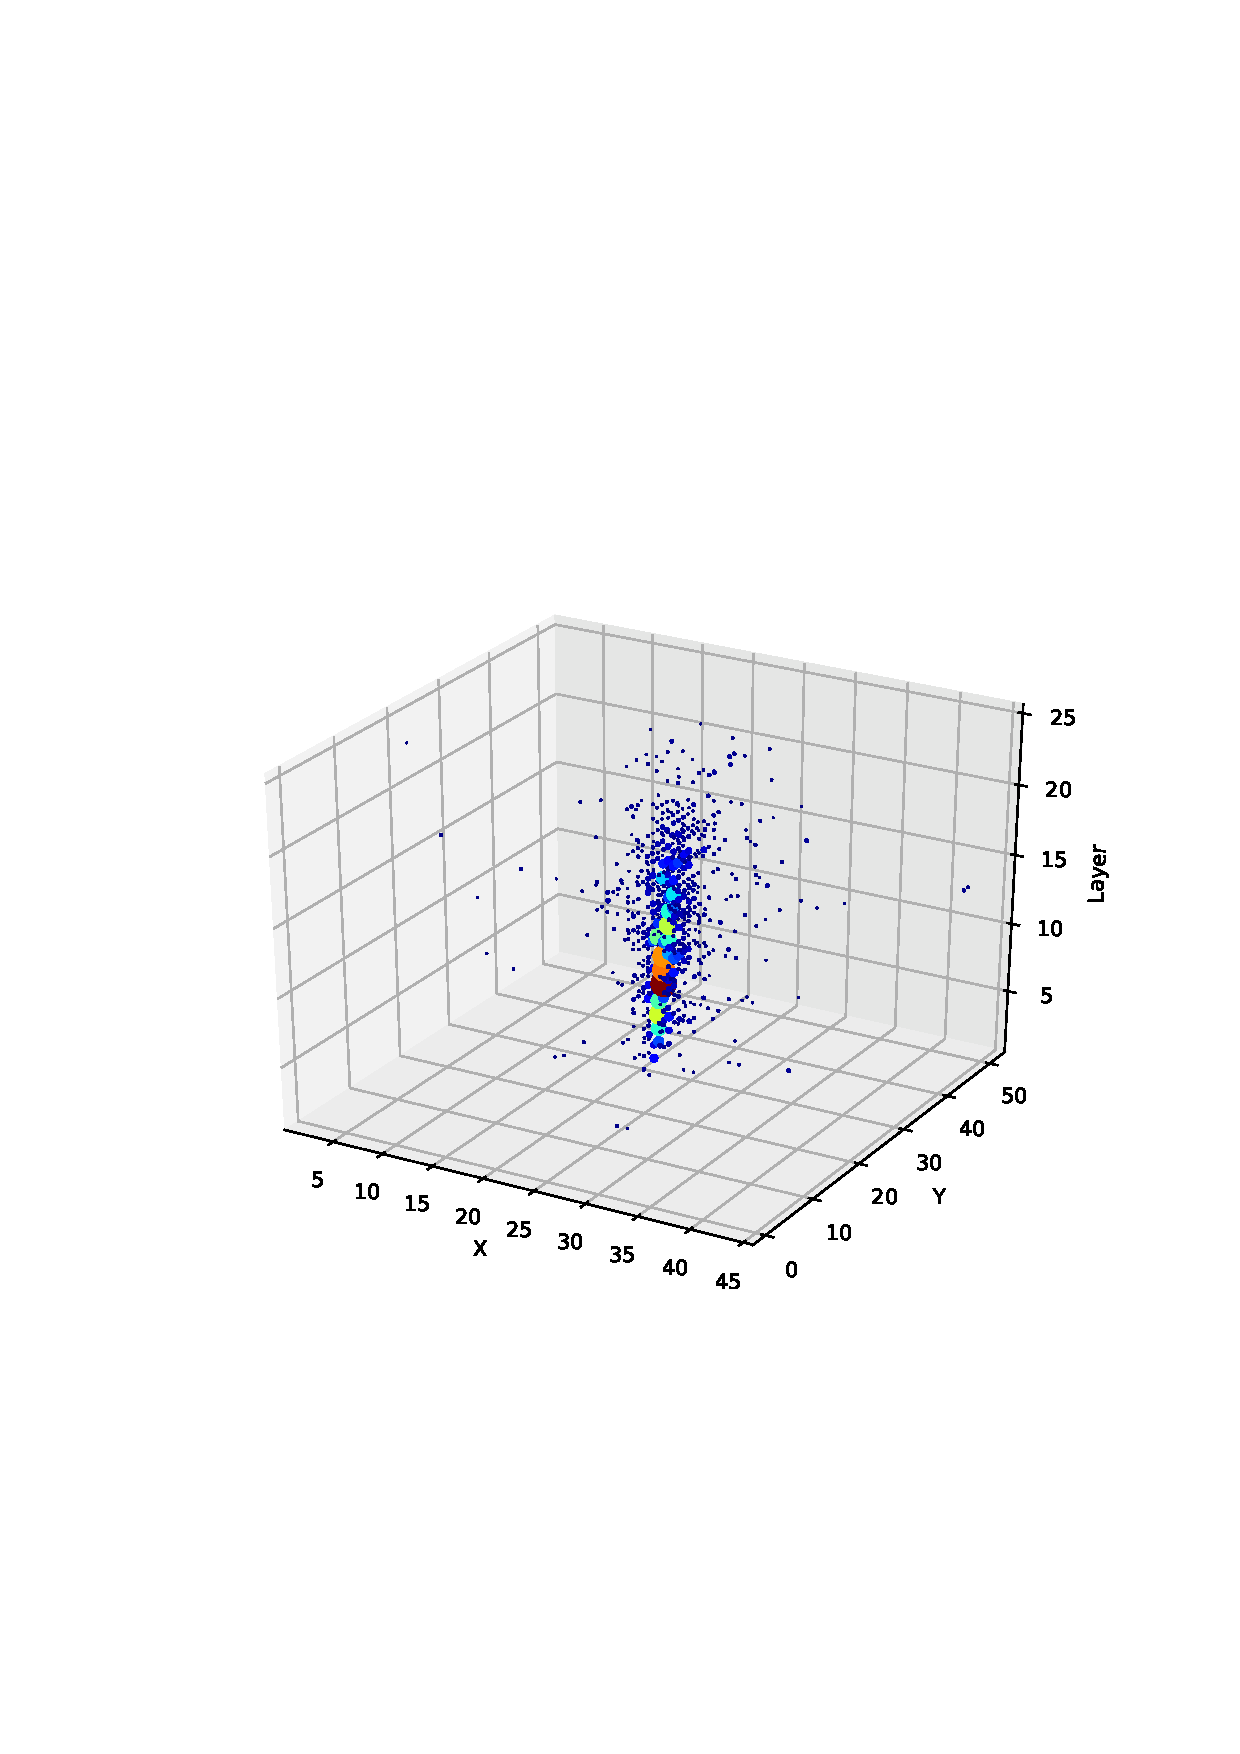
\includegraphics[width=0.45\textwidth]{images/Gamma_ECAL.pdf}
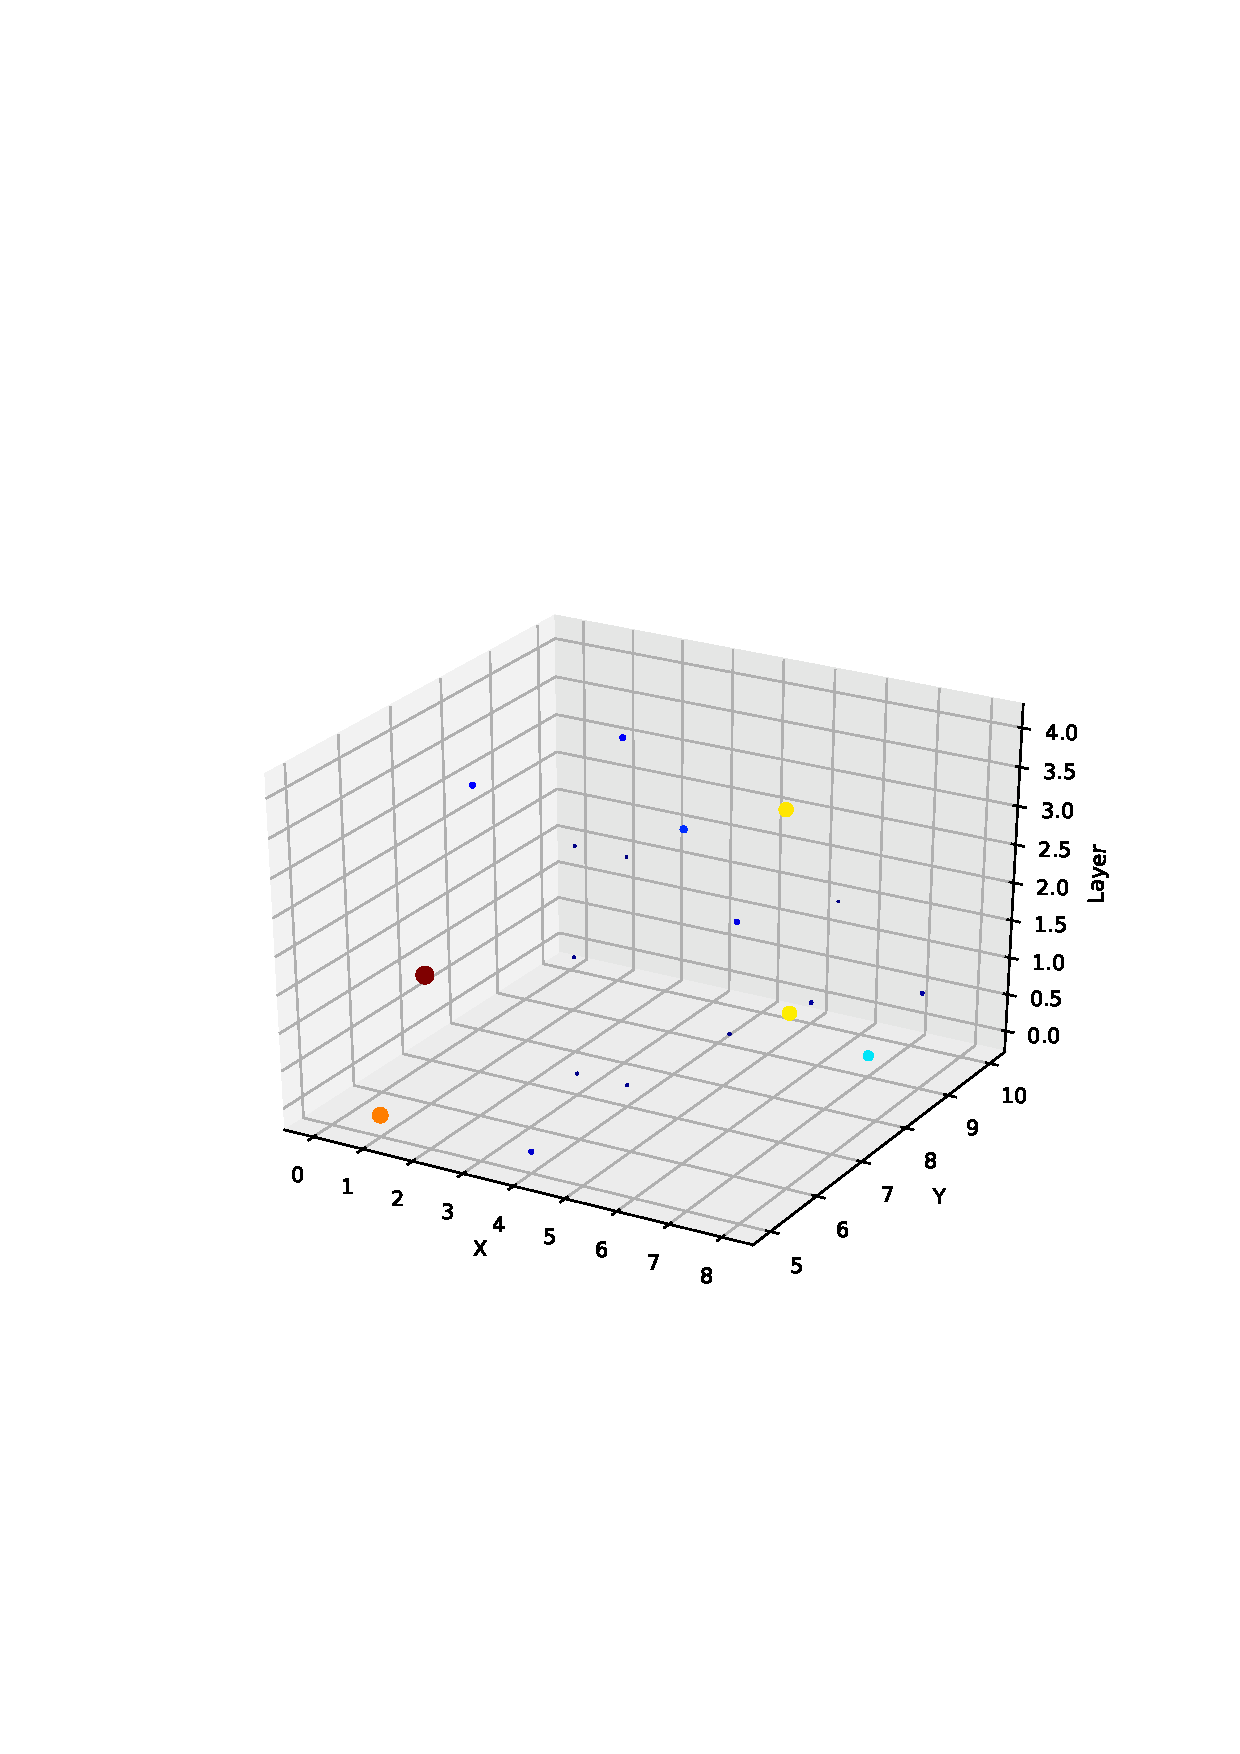
\includegraphics[width=0.45\textwidth]{images/Gamma_HCAL.pdf} \\
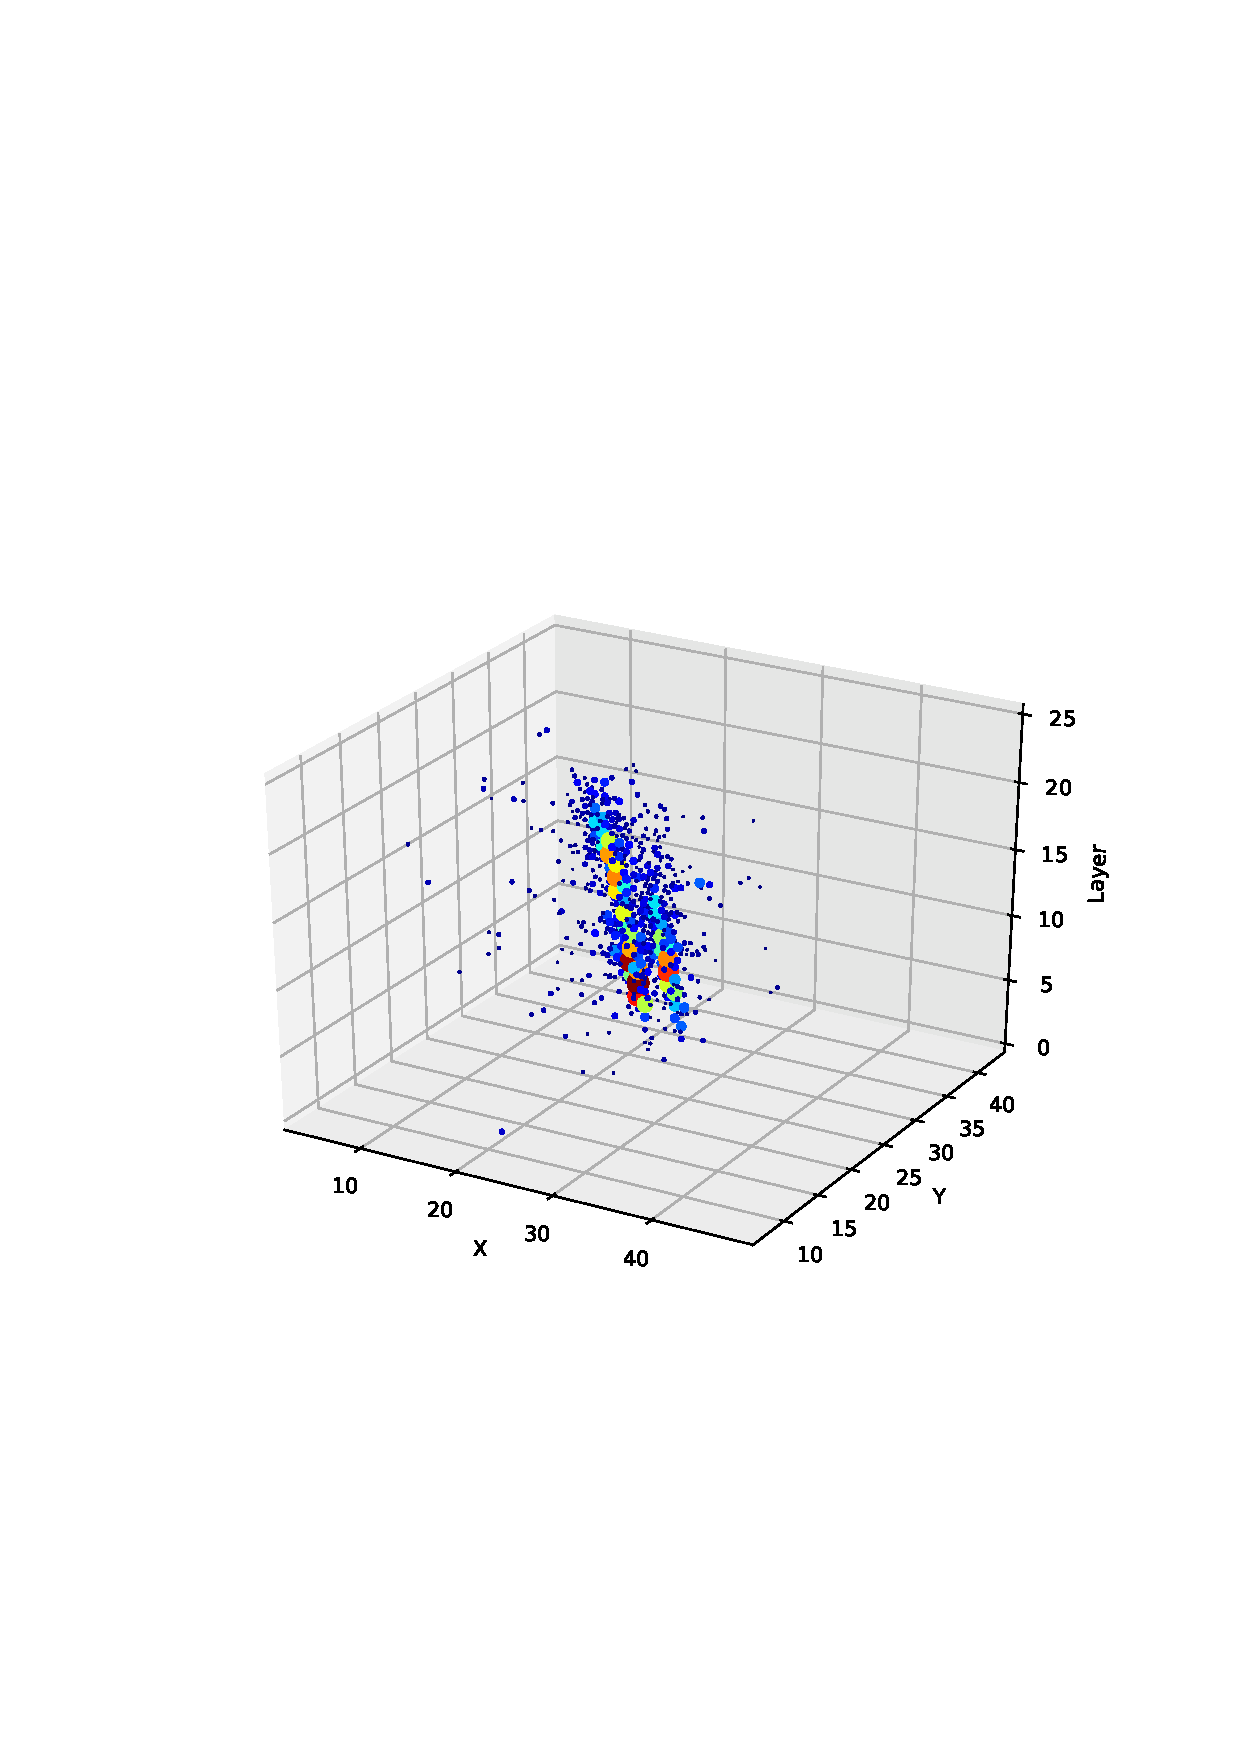
\includegraphics[width=0.45\textwidth]{images/Pi0_ECAL.pdf}
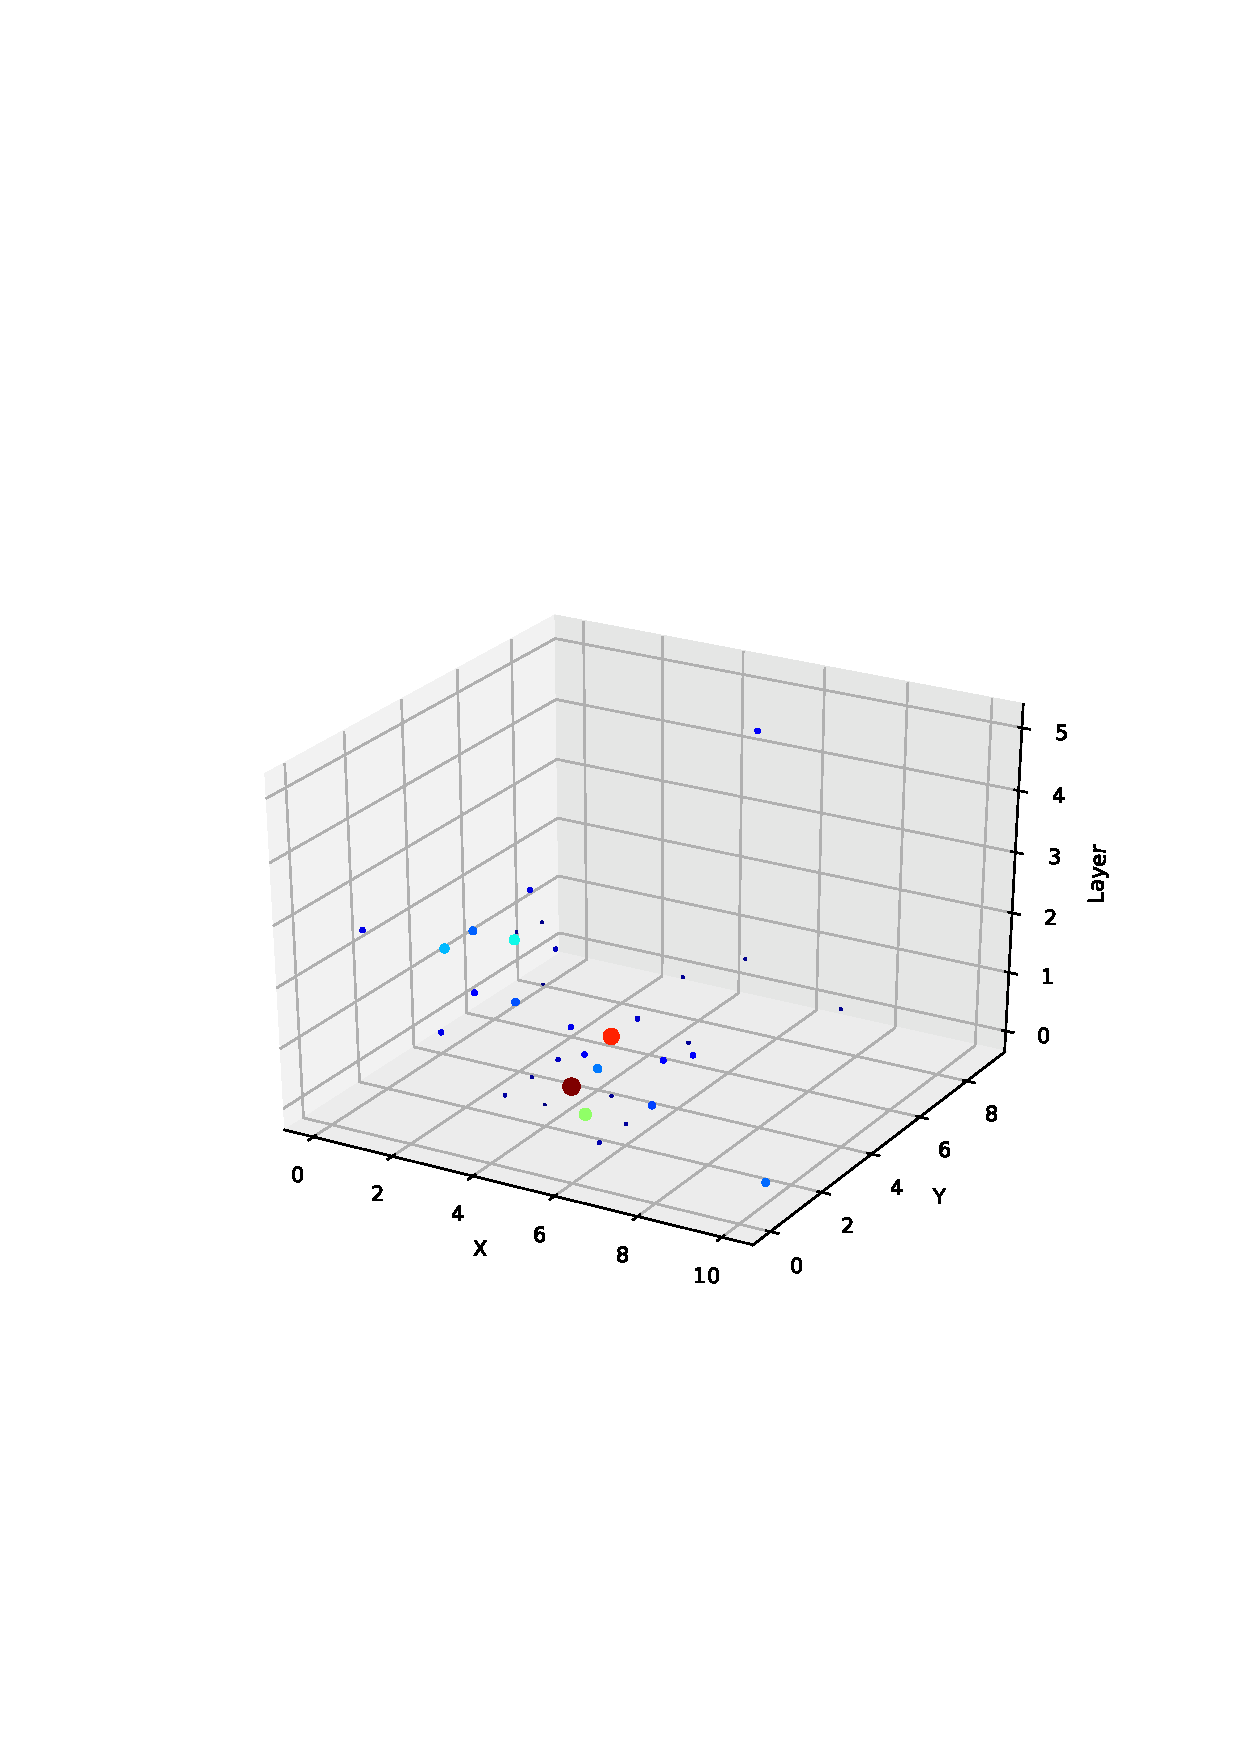
\includegraphics[width=0.45\textwidth]{images/Pi0_HCAL.pdf}
\caption{3D image of a photon (top) and neutral pion (bottom) shower in ECAL (left) and HCAL (right).}
\label{fig:sample}
\end{figure*}

%%%%%%%%%%%%%%%%%

\begin{figure}[htbp]
\centering
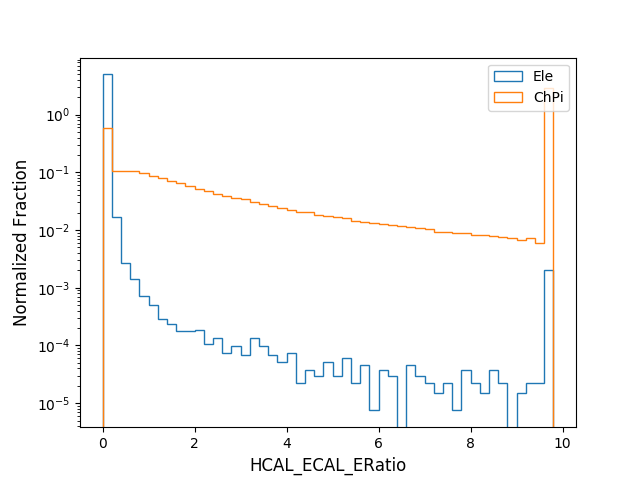
\includegraphics[width=0.3\textwidth]{images/ratios.png}
\includegraphics[width=0.3\textwidth]{images/zoom_ratios.png}
\caption{HCAL/ECAL energy ratios for electrons and charged pions. The bottom plot is a zoomed-in version of the top plot.}
\label{fig:HE_ratio}
\end{figure}

\begin{figure}[htbp]
\centering
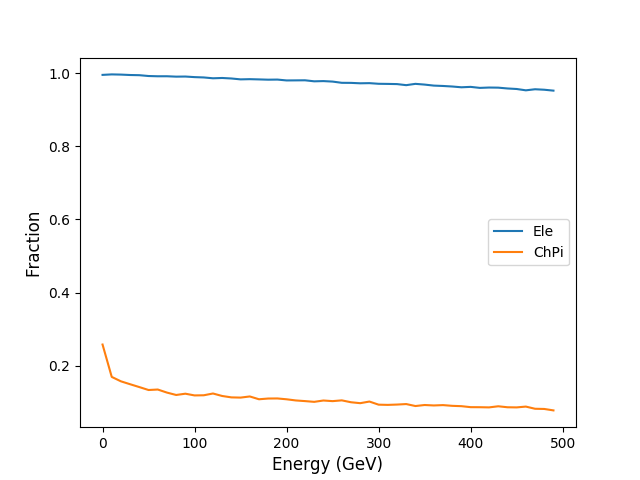
\includegraphics[width=0.3\textwidth]{images/ratio_cut_vs_energy.png}
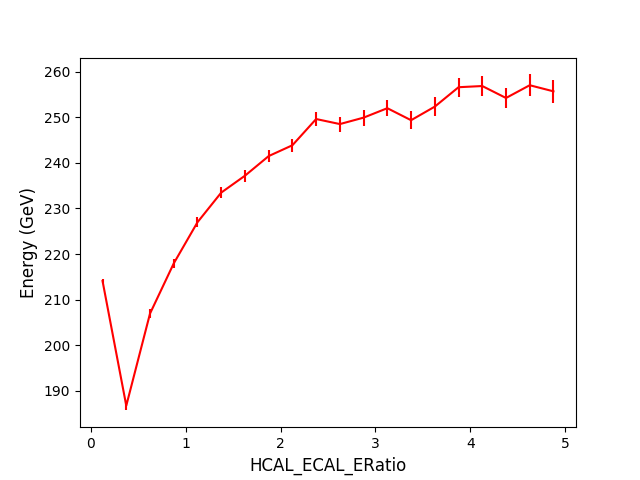
\includegraphics[width=0.3\textwidth]{images/mean_energy_vs_ratio.png}
\caption{Fractions of electrons and charged pions passing a HCAL/ECAL energy selection at various particle energies (top). The mean charged pion energy at each energy ratio (bottom).}
\label{fig:HE_ratio_energy}
\end{figure}

\begin{figure}[htbp]
\centering
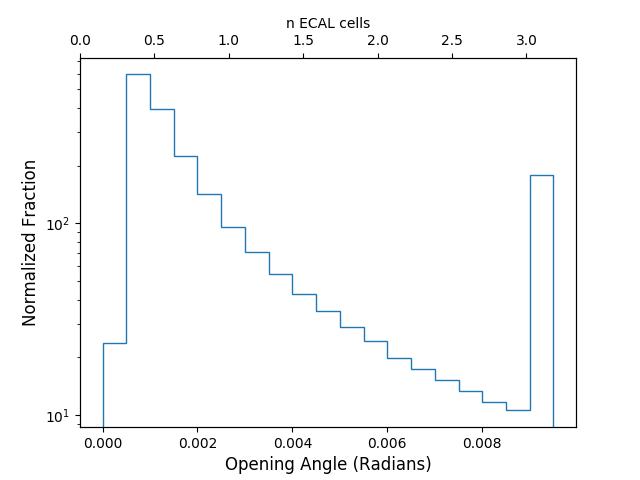
\includegraphics[width=0.3\textwidth]{images/zoom_opening_angles.png}
\caption{Opening angle distribution for neutral pions decaying into two photons.}
\label{fig:opening_angle}
\end{figure}

\begin{figure}[htbp]
\centering
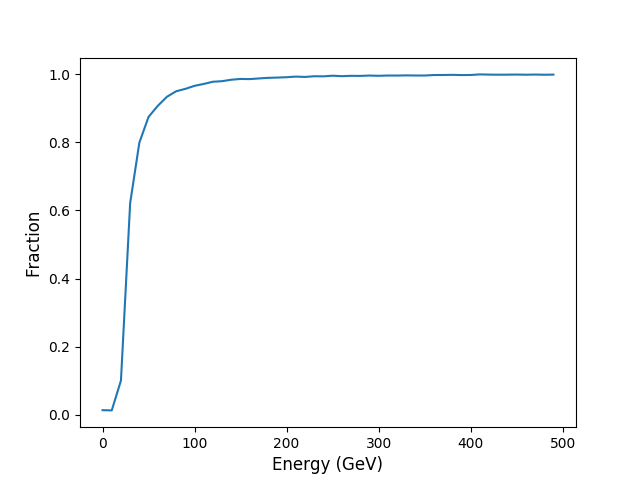
\includegraphics[width=0.3\textwidth]{images/opening_angle_cut_vs_energy.png}
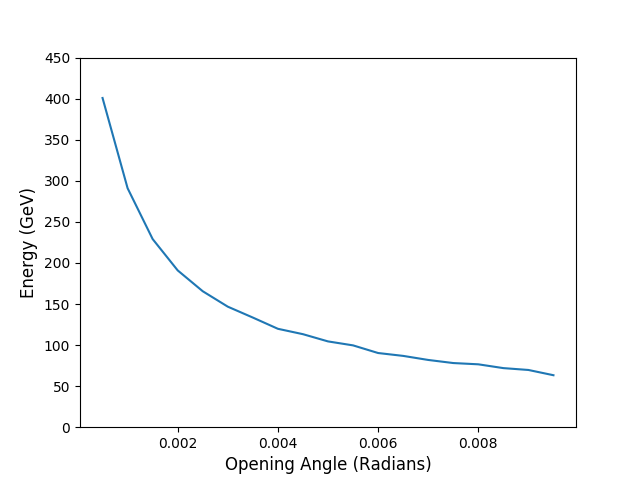
\includegraphics[width=0.3\textwidth]{images/mean_energy_vs_opening_angle.png}
\caption{The fraction of photons and neutral pions passing an opening angle < 0.01 radian selection at various particle energies (top). The mean neutral pion energy at each opening angle (bottom).}
\label{fig:opening_angle_energy}
\end{figure}

We apply a task-dependent filtering of the REC dataset, in order to select the subset of examples for which the task at hand is not trivial. For instance, distinguishing a generic pion from a generic electron is an easy task, and can be accomplished with high accuracy by looking at the HCAL/ECAL energy ratio. On the other hand, it is difficult to distinguish a generic electron from a pion that has a small HCAL/ECAL energy ratio. Thus, we ignore charged-pion showers with a large HCAL/ECAL energy ratio. To be more specific, we see in Figure~\ref{fig:HE_ratio} that the ratio of total ECAL energy to total HCAL energy is very different for electrons and charged pions, with the heavier charged pions tending to leave little energy in the ECAL. In order to make the particle-identification task more challenging, we only consider showers with HCAL/ECAL < 0.1 cut. The results of this selection are shown in Figure~\ref{fig:HE_ratio_energy}. We can see that this selection favors mostly low-energy charged pions, which tend to leave more of their energy in the ECAL rather than punching through to the HCAL. Discriminating accurately between electrons and charged pions in this range is thus crucial for compressed-mass physics analyses, where we search for decay products with low energy.

Photons and neutral pions are more similar to each other. The easily distinguishable events are mostly due to the fact that neutral pions decay into two photons which are separated by a small angle. If the pion has a low energy, the opening angle between the two photons is larger and the shower is easily identified as originating from a neutral pion. High-energy neutral pions produce more collimated photon pairs, which are more easily mistaken as a single high-energy photon. The opening angle distribution for neutral pions is shown in Figure~\ref{fig:opening_angle}. In order to limit the study to the most challenging case, we filter the neutral-pion dataset by requiring the opening angle between the two photons to be smaller than 0.01 radian.  The effect of  this requirement on the otherwise uniform energy distribution is shown in Figure~\ref{fig:opening_angle_energy}. As expected, the selection mostly removes low-energy neutral pions. 

%Generating events with these filters applied turned out to be a significant use of computing resources, especially when it came to the charged pion samples. Applying the HCAL/ECAL < 0.1 selection meant that we needed to generate several hundred times as many charged pion events as we would have needed without the filter.

The ECAL and HCAL 3D arrays are passed directly to our neural networks. We also compute a set of expert features, as described in Ref.~\cite{NIPS}. These features are used to train alternative benchmark algorithms (see Appendices~\ref{app:BDT}~and~\ref{app:regression_baseline}), representing currently-used ML algorithms in HEP.

\section{Classification and Regression}

\section{End-to-End Particle Reconstruction}
\label{sec:reco}

This section describes the use of a deep neural network to accomplish an end-to-end particle reconstruction task. The model consists of a neural architecture which simultaneously performs both particle classification and energy regression. This combined network is trained using the ECAL and HCAL cell arrays as well as the total ECAL energy and total HCAL energy as inputs. The training loss function is written as the sum of a binary cross entropy for particle identification and a mean-square error loss for energy regression. Through experimentation, we found that multiplying the energy loss by a factor of 200 gave the best results, as it was easier to quickly achieve low loss values for energy regression.

We compare three different architectures for our reconstruction model, each trained using calorimeter cell-level information as inputs:
\begin{itemize}
\item A dense (i.e, fully connected) neural network (DNN).
\item A 3D convolutional network (CNN).
\item A network based on GoogLeNet (GN)~\cite{GoogLeNet}, using layers of inception modules.
\end{itemize}

In order to compare the model performance to a typical state-of-the-art particle reconstruction algorithm, we also consider the following alternatives:
\begin{itemize}
    \item A feature-based BDT (see Appendix~\ref{app:BDT}) for the classification task.
    \item A linear regression for the regression task.
    \item A BDT for the regression task (for more info on regression baselines see Appendix~\ref{app:regression_baseline}).
\end{itemize}

In a previous study~\cite{NIPS}, we compared the classification accuracy obtained with a neural model taking as input the energy cells, a feature-based neural models, and a feature-based BDTs. In that context, we demonstrated that feature-based BDTs and neural networks perform equally well, and are both equally capable of correctly classify particles from a small set of calculated features. 
%Increases in classification accuracy are mostly due to the neural architecture's ability to extract meaning from a much larger input dataset, the calorimeter cell-level energy information. For this reason, w
We do not compare feature-based neural networks in this paper, and use feature-based BDTs to represent the current state-of-the-art classification algorithms.

\subsection{Deep Network Models}

The three ML models take as input the ECAL and HCAL 3D energy arrays of the REC dataset (see Section~\ref{sec:data}), together with the total energies recorded in ECAL and in HCAL (i.e., the sum of the values stored in the 3D arrays), as well as the estimated $\phi$ and $\eta$ angles of the incoming particle, calculated using the collision origin and the barycenter of the event. The architecture of each model is defined with a number of floating parameters (e.g. number of hidden layers), which are refined through a hyperparameter optimization, as described in Section~\ref{sec:hpscan}. Each model returns three numbers. After applying a softmax activation, two of these elements are interpreted as the classification probabilities of the current two-class problem. The third output is interpreted as the energy of the particle.

Here we describe in detail the three model architectures:

\begin{itemize}
    \item In the DNN model we first flatten our ECAL and HCAL inputs into 1D arrays. We then concatenate these array along with the total ECAL energy, total HCAL energy, estimated $\phi$, and estimated $\eta$, for an array of total size $25 \times 25 \times 25 + 11 \times 11 \times 60 + 4 = 22889$ inputs. This array is fed as input to the first layer of the DNN, followed by a number of hidden layers each followed by a ReLU activation function and a dropout layer. The number of neurons per hidden layer and the dropout probability are identical for each relevant layer. The number of hidden layers, number of hidden neurons per layer, and dropout rate are hyperparameters, tuned as described in the next session.  Finally, we take the output from the last dropout layer, append the total energies and estimated angles again, and feed the concatenated array into a final hidden layer, which results in a three-element output. 
    \item The CNN architecture consists of one 3D convolutional layer for each of the ECAL and HCAL inputs, each followed by a ReLU activation function and a max pooling layer of kernel size $2 \times 2 \times 2$. The number of filters and the kernel size in the ECAL convolutional layer are treated as optimized hyperparameter (see next session). The HCAL layer is fixed at 3 filters with a kernel size of $2 \times 2 \times 6$. The two outputs are then flattened and concatenated along with the total ECAL and HCAL energies, as well as the estimated $\phi$ and $\eta$ coordinates of the incoming particle. The resulting 1D array is passed to a sequence of dense layers each followed by a ReLU activation function and dropout layer, as in the DNN model. The number of hidden layers and the number of neurons on each layer are considered as hyperparameters to be optimized. The output layer consists of three numbers, as for the DNN model. We found that adding additional convolutional layers to this model beyond the first had little impact on performance. This may be because a single layer is already able to capture important information about localized shower structure, and reduces the dimensionality of the event enough where a densely connected net is able to do the rest.
    \item The third model uses elements of the GoogLeNet~\cite{GoogLeNet} architecture. This network processes the ECAL input array with a 3D convolutional layer with 192 filters, a kernel size of 3 in all directions, and a stride size of 1. The result is batch-normalized and sent through a ReLU activation function. This is followed by a series of inception and MaxPool layers of various sizes, with the full architecture described in Appendix~\ref{app:GoogLeNet}. The output of this sequence is concatenated to the total ECAL energy, the total HCAL energy, the estimated $\phi$ and $\eta$ coordinates, and passed to a series of dense layers like in the DNN architecture, to return the final three outputs. The number of neurons in the final dense hidden layer is the only architecture-related hyperparameter for the GN model. Due to practical limitations imposed by memory constraints, this model does not take the HCAL 3D array as input. This limitation has a small impact on the model performance, since the ECAL array carries the majority of the relevant information for the problems at hand (see Appendix~\ref{app:classification_HCAL}).
\end{itemize}

On all models, the regression task is facilitated by using skip connections to directly append the input total ECAL and HCAL energies to the last layer. The impact of this architecture choice on regression performance is described in Appendix~\ref{app:skip_connections}. In addition to using total energies, we also tested the possibility of using 2D projections of the input energy arrays, summing along the $z$ dimension (detector depth). This choice resulted in worse performance (see Appendix~\ref{app:z_sum_regression}) and was discarded.

\subsection{Hyperparameter Scans}
\label{sec:hpscan}

In order to determine the best architectures for the end-to-end reconstruction models, we scanned over a hyperparameter space for each architecture. Learning rate and decay rate were additional hyperparameters for each architecture. For simplicity, we used classification accuracy for the $\gamma$ vs. $\pi^0$ problem as a metric to determine the overall best hyperparameter set for each architecture. This is because a model optimized for this task was found to generate good results for the other three tasks as well, and because $\gamma$ vs. $\pi^0$ classification was found to be the most difficult problem.

Each hyperparameter point was scanned ten times, in order to obtain an estimate of the uncertainty associated with each quoted performance value. For each scan point, the DNN and CNN architectures trained on 400,000 events, using another sample of 400,000 events for testing. DNN and CNN scan points trained for three epochs each, taking about seven hours each. GN trained on 100,000 events and tested on another 100,000. Due to a higher training time, each GN scan point only trained for a single epoch, taking about twenty hours.

For CNN and DNN training, we used batches of 1,000 events when training. However, due to GPU memory limitations, we could not do the same with GN. Instead, we split each batch into 100 minibatches of ten events each. A single minibatch was loaded on the GPU at a time, and gradients were added up after back-propagation. Only after the entire batch was calculated did we update network weights using the combined gradients.

The best settings were found to be as follows:
\begin{itemize}
    \item For DNN, 4 hidden layers, 512 neurons per hidden layer, a learning rate of 0.0002, decay rate of 0, and a dropout probability of 0.04.
    \item For CNN, 4 hidden layers and 512 neurons per hidden layer, a learning rate of 0.0004, decay rate of 0, a dropout probability of 0.12, 6 ECAL filters with a kernel size of $6 \times 6 \times 6$.
    \item For GN, 1024 neurons in the hidden layer, 0.0001 learning rate, and 0.01 decay rate. 
\end{itemize}
%For CNN and GN, a very mild dependence on the number of neurons per hidden layer is observed. 

\begin{figure*}[htbp]
\centering
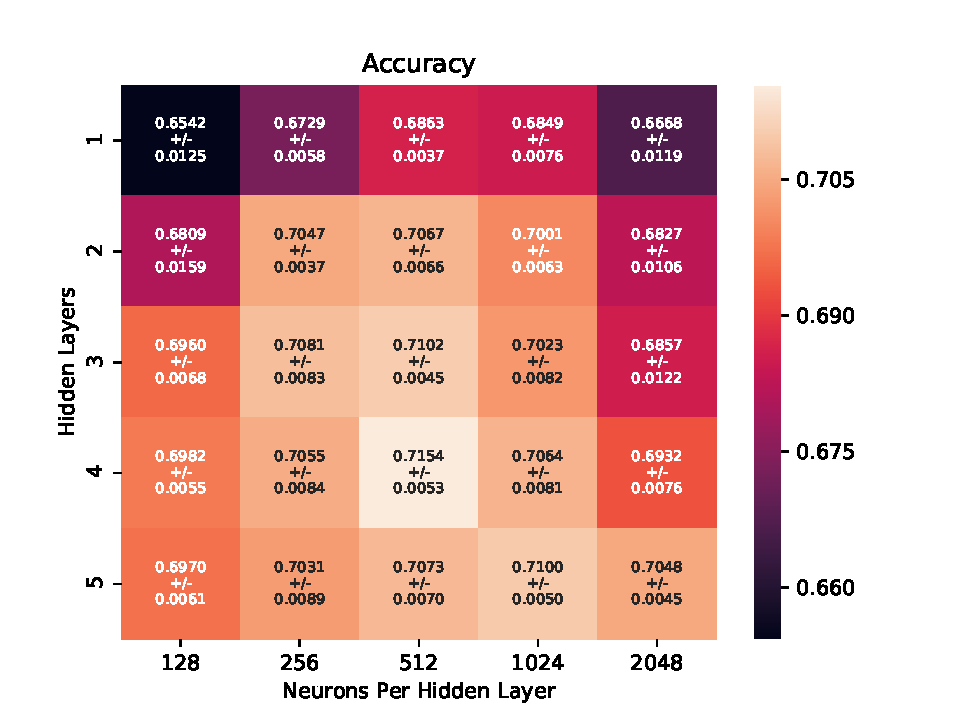
\includegraphics[width=0.45\textwidth]{images/DNN_hl_nhl}
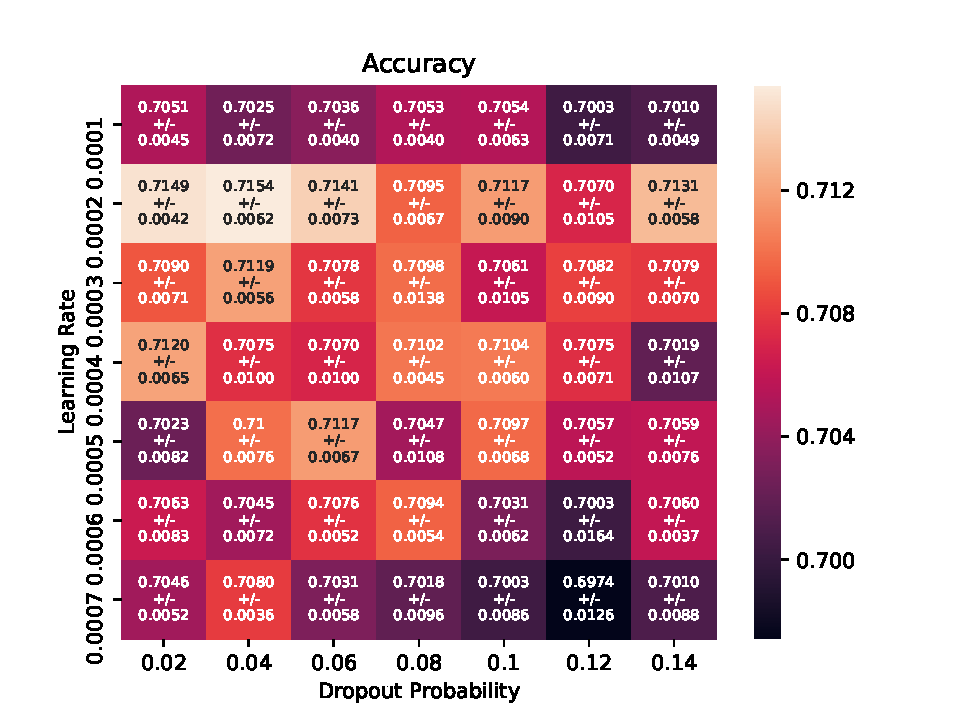
\includegraphics[width=0.45\textwidth]{images/DNN_lr_dp} \\
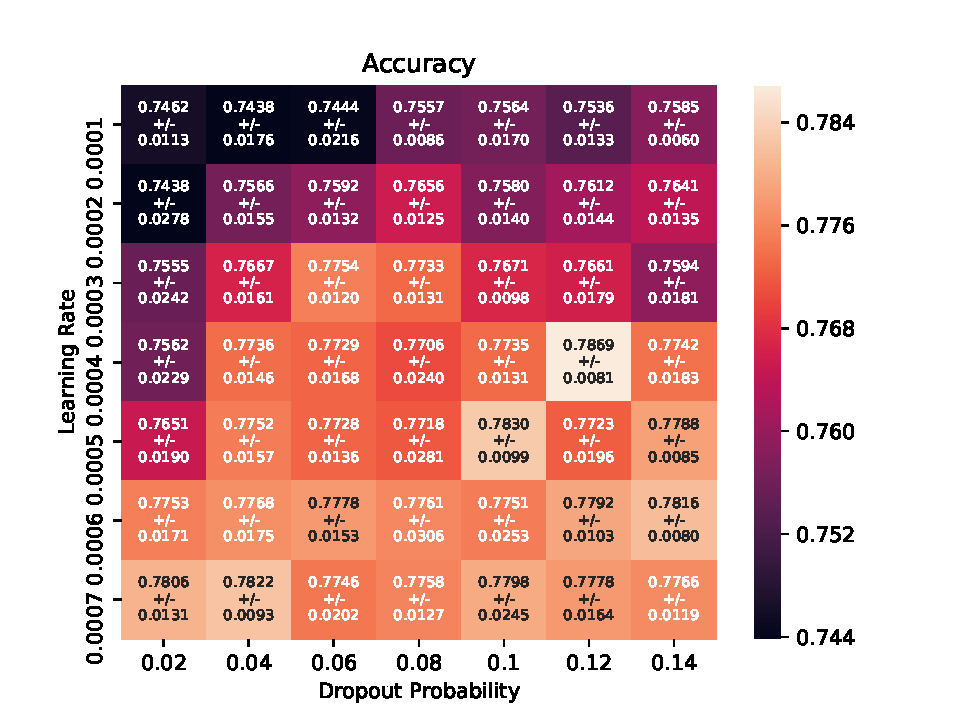
\includegraphics[width=0.45\textwidth]{images/CNN_lr_dp}
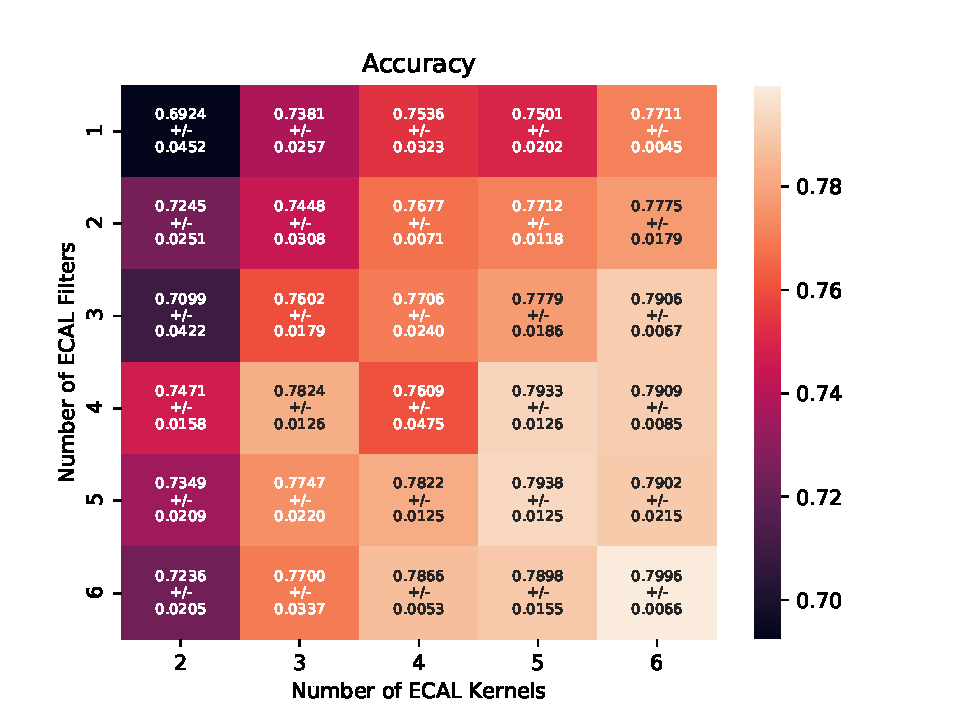
\includegraphics[width=0.45\textwidth]{images/CNN_nECALfilt_nECALkern} \\
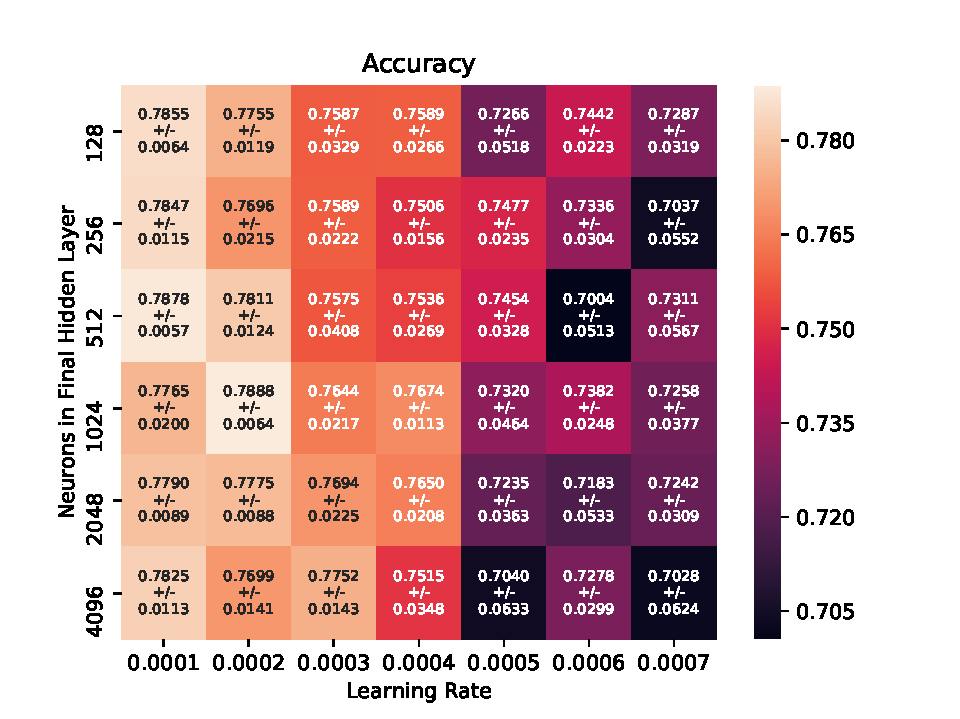
\includegraphics[width=0.45\textwidth]{images/GN_nhl_lr}
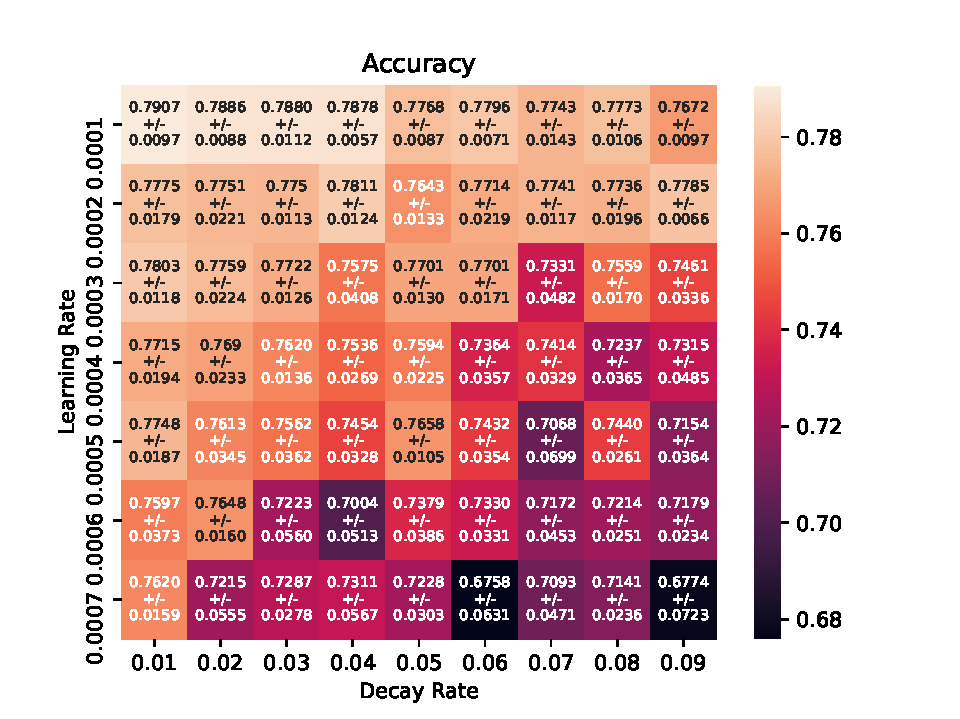
\includegraphics[width=0.45\textwidth]{images/GN_lr_dr}
\caption{Selected hyperparameter scan results for DNN (top), CNN (center), and GN (bottom). In each figure, the classification accuracy is displayed as a function of the hyperparameters reported on the two axes.}
\label{fig:scan_hyperparameter}
\end{figure*}

Selected hyperparameter scan slices are shown in Figure~\ref{fig:scan_hyperparameter}. 
These 2D scans were obtained setting all values besides the two under consideration (i.e., those on the axes) to be fixed at default values: a dropout rate of 0.08, a learning rate of 0.0004, a decay rate of 0.04, three dense layers for CNN and DNN, and 512 neurons per hidden layer. For GN, the default number of ECAL filters was 3, with a kernel size of 4.
%An ECAL window size of 25 was used in all instances, to allow fair comparison between DNN, CNN, and GN, as larger ECAL sizes posed a memory problem when training GN.

After performing the hyperparameter scan, we trained each architecture using its optimal hyperparameters for a greater number of epochs. The evolution of the training and validation accuracy as a function of the batch number for these extended trainings is shown in Figure~\ref{fig:training_curves_comparison_gamma_pi0}.

\begin{figure}[htbp]
\centering
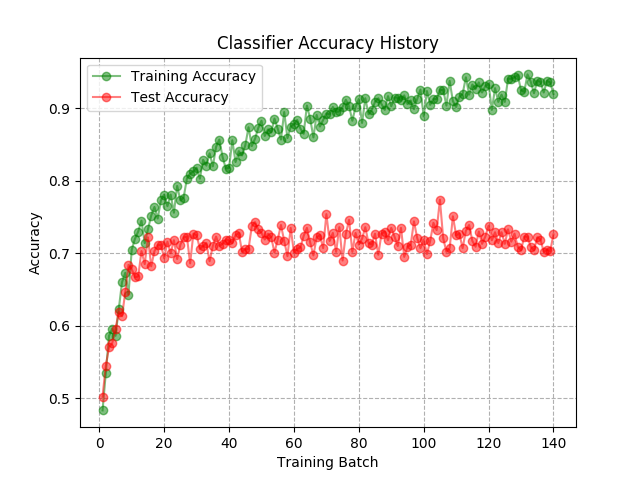
\includegraphics[width=0.42\textwidth]{images/DNN_accuracy_batches_long}
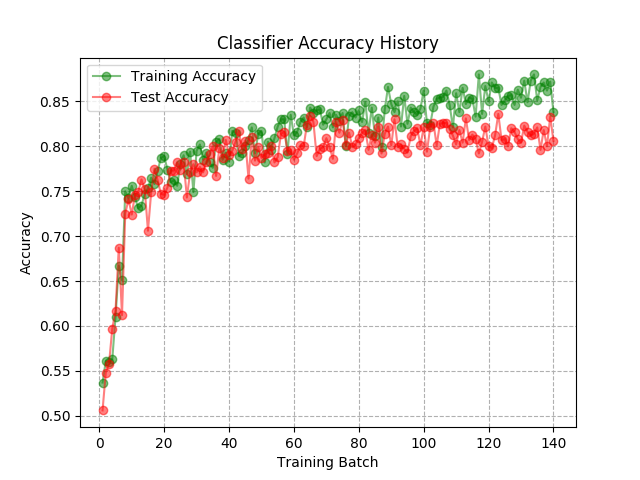
\includegraphics[width=0.42\textwidth]{images/CNN_accuracy_batches_long}
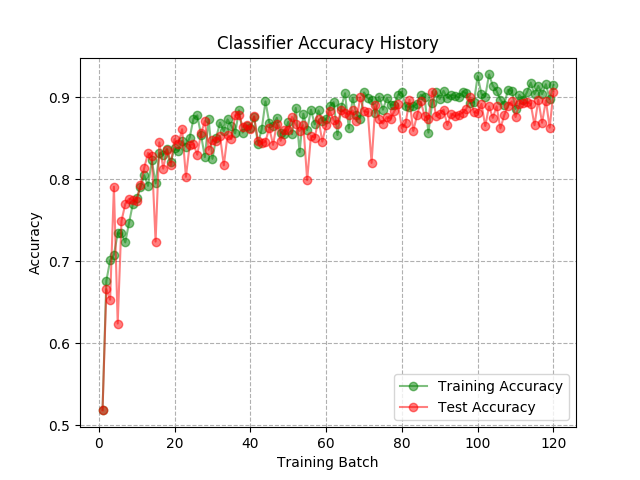
\includegraphics[width=0.42\textwidth]{images/GN_accuracy_batches_long}
\caption{Training curves for best DNN (top), CNN (middle), and GN (bottom) hyperparameters, trained on variable-angle $\gamma$/$\pi^0$ samples. We see that the DNN over-trains quickly and saturates at a relatively low accuracy, while the CNN takes longer to over-train and reaches a higher accuracy, and GN performs best of all. Each 400 batches corresponds to a single epoch.}
\label{fig:training_curves_comparison_gamma_pi0}
\end{figure}

\subsection{Results}

We apply the best architectures described in the previous section separately to our electron vs. charged pion and photon vs. neutral pion reconstruction problems.

\subsubsection{Classification Performance}
\label{sec:classification}

Figure~\ref{fig:architectures_ROC_comparisons} shows ROC curve comparisons for the two classification tasks. As expected, the electron vs. charged pion classification problem was found to be a simple task, resulting in an area under the curve (AUC) close to $100\%$. For a baseline comparison, the curve obtained for a BDT (see Appendix~\ref{app:BDT}) is also shown. This BDT was optimized using the {\it scikit-optimize} package~\cite{skopt}, and was trained using high-level features computed from the raw 3D arrays. It represents the performance of current ML approaches on these problems.

\begin{figure}[htbp]
\centering
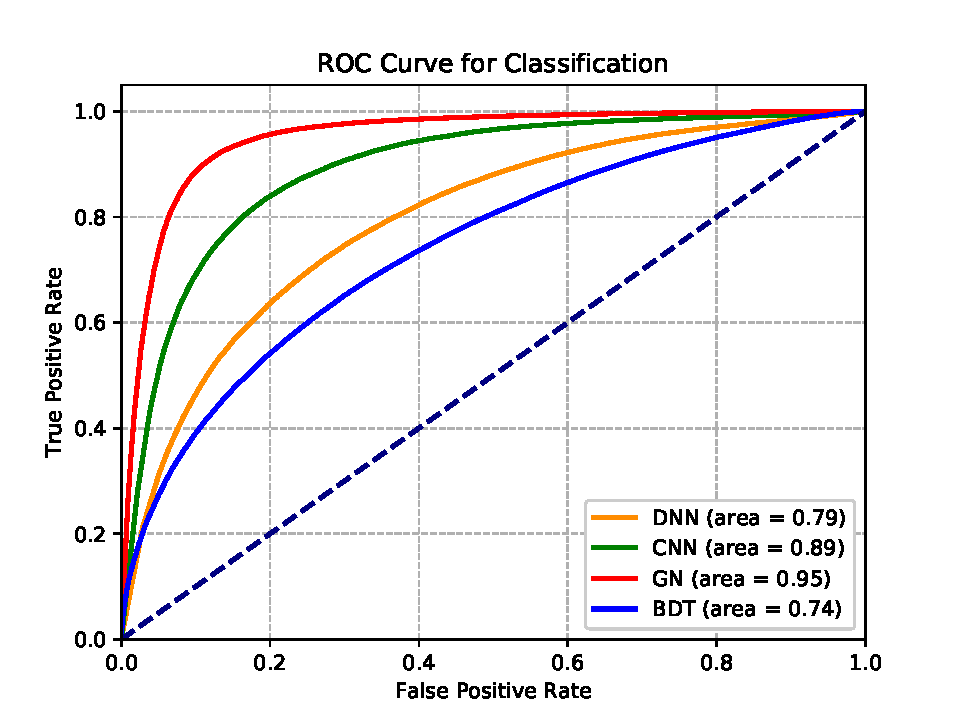
\includegraphics[width=0.45\textwidth]{images/architectures_ROC_comparison_gamma_pi0_long}
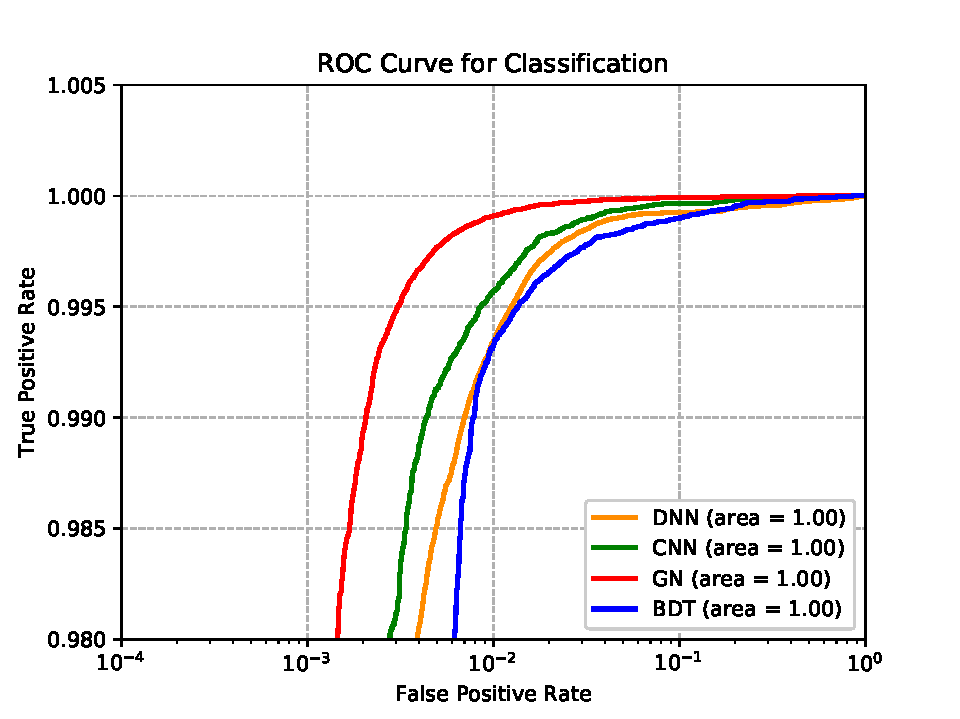
\includegraphics[width=0.45\textwidth]{images/architectures_ROC_comparison_ele_chpi_xlog}
\caption{ROC curve comparisons for $\gamma$ vs. $\pi^0$ (top) and $e$ vs. $\pi^\pm$ (bottom) classification using different neural network architectures. Samples include particle energies from 10 to 510 GeV, and an inclusive $\eta$ range.}
\label{fig:architectures_ROC_comparisons}
\end{figure}

The ML models outperform the BDT, with the GN reaching the best classification performance on both problems. Figure~\ref{fig:accuracy_bins} shows the best-model performance as a function of the energy and $\eta$ of the incoming particle, for the photon vs. neutral pion and the electron vs. charged pion problems. These figures show that classification accuracy is maintained over a wide range of particle energies and angles. The models appear to perform a bit worse at higher energies for the photon vs. neutral pion case, due to the fact that the pion to two photon decay becomes increasingly collimated at higher energies. Similarly, the performance is slightly worse when particles impact the detector perpendicularly than when they enter at a wide angle, because the shower cross section on the calorimeter inner surface is reduced at $90^{\mathrm o}$, making it harder to distinguish shower features.

\begin{figure*}[htbp]
\centering
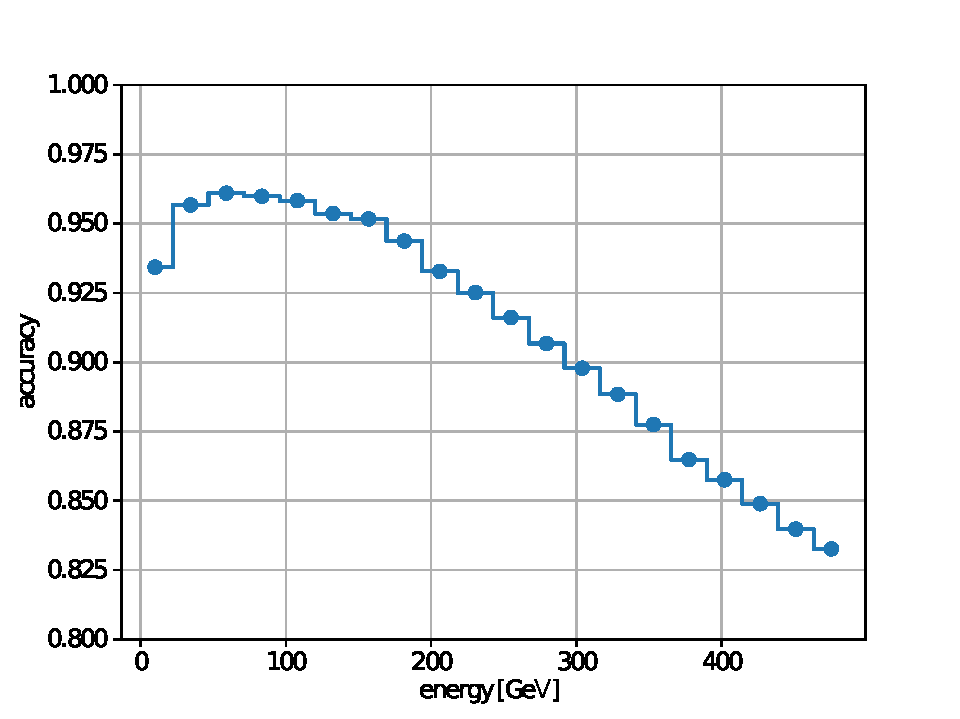
\includegraphics[width=0.45\textwidth]{images/gamma_pi0_accuracy_energy_bins.pdf}
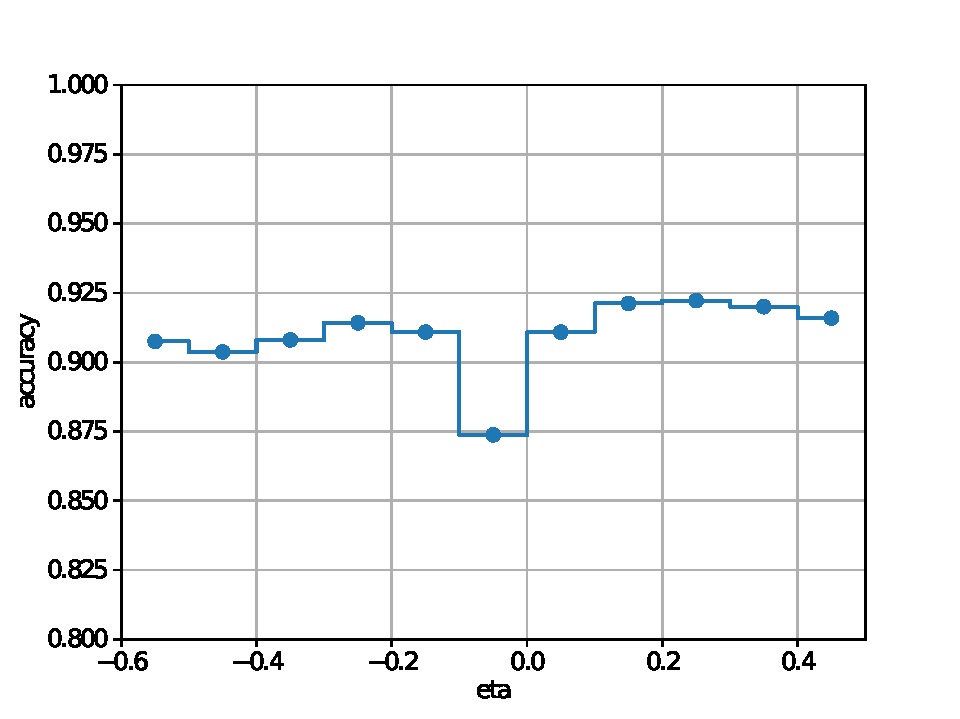
\includegraphics[width=0.45\textwidth]{images/gamma_pi0_accuracy_eta_bins.pdf} \\
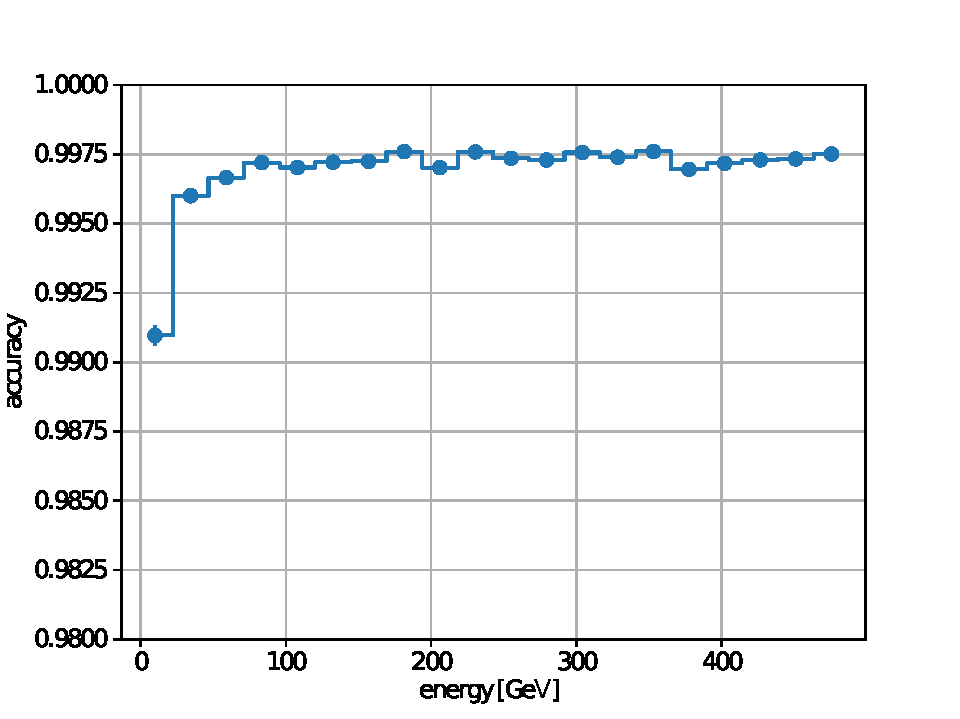
\includegraphics[width=0.45\textwidth]{images/ele_chpi_accuracy_energy_bins.pdf}
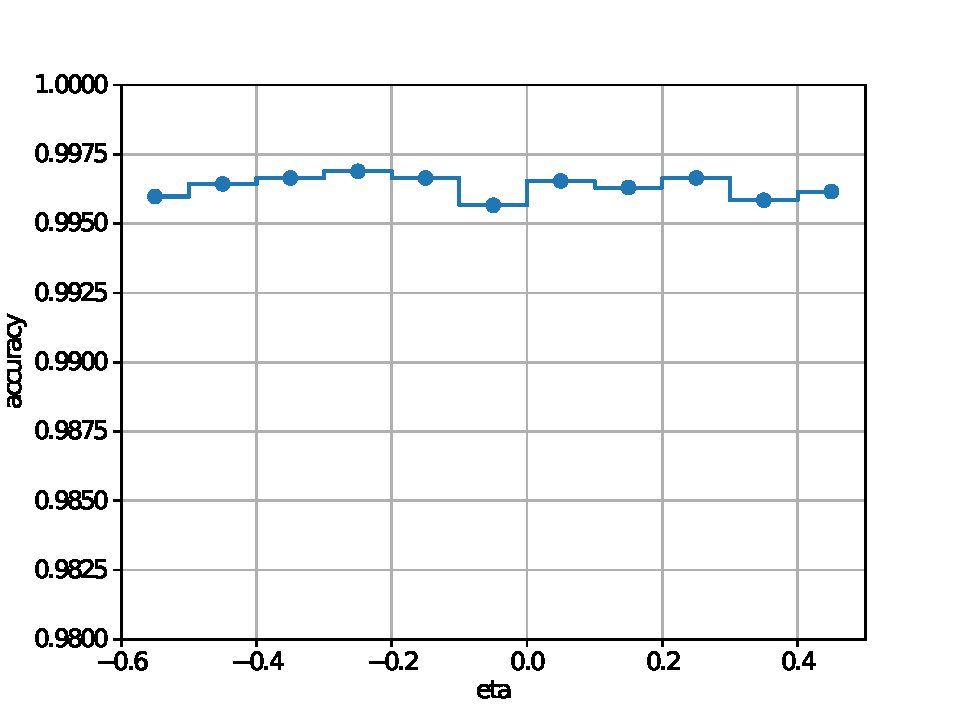
\includegraphics[width=0.45\textwidth]{images/ele_chpi_accuracy_eta_bins.pdf}
\caption{Classification accuracy of best performing network for $\gamma$ vs. $\pi^0$ (top) and $e$ vs. $\pi^\pm$ (bottom), in bins of energy (left) and $\eta$ (right).}
\label{fig:accuracy_bins}
\end{figure*}


%%%% REGRESSION
\subsubsection{Regression Performance}
\label{sec:regression}

Figure~\ref{fig:reg_dnn_vs_cnn_variable} shows the energy regression performance for each particle type, obtained from the end-to-end reconstruction architectures. In this case, we compare against a linear regression algorithm and a BDT (labelled as "XGBoost") representing the current state-of-the-art, as described in Appendix~\ref{app:regression_baseline}. 

\begin{figure*}[htbp]
\centering
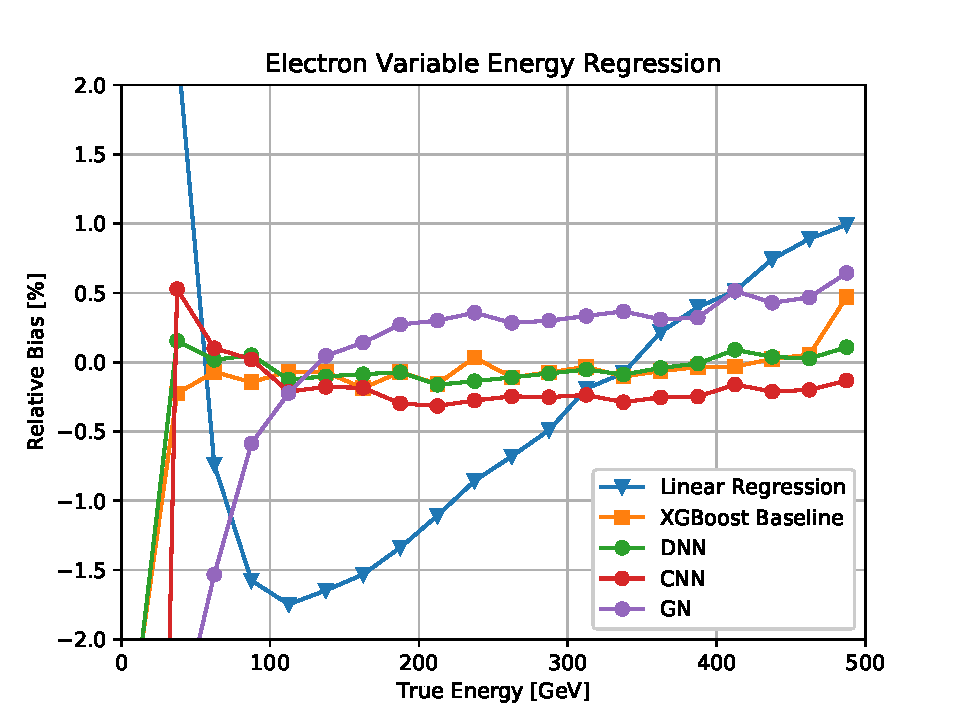
\includegraphics[width=0.38\textwidth]{images/bias_vs_E_Ele_variable}
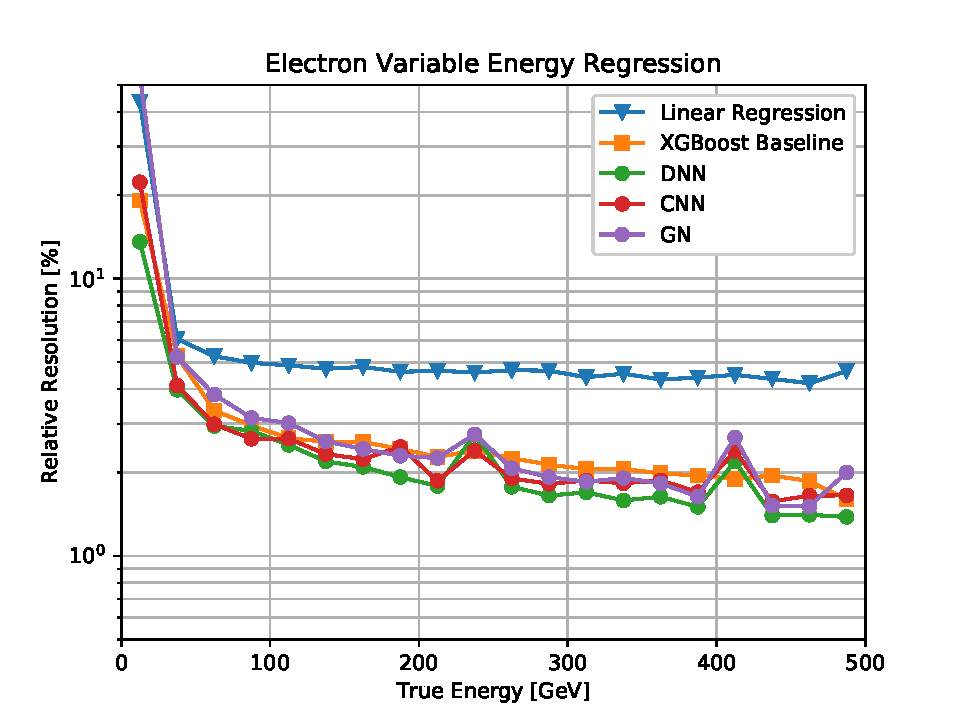
\includegraphics[width=0.38\textwidth]{images/res_vs_E_Ele_variable} \\
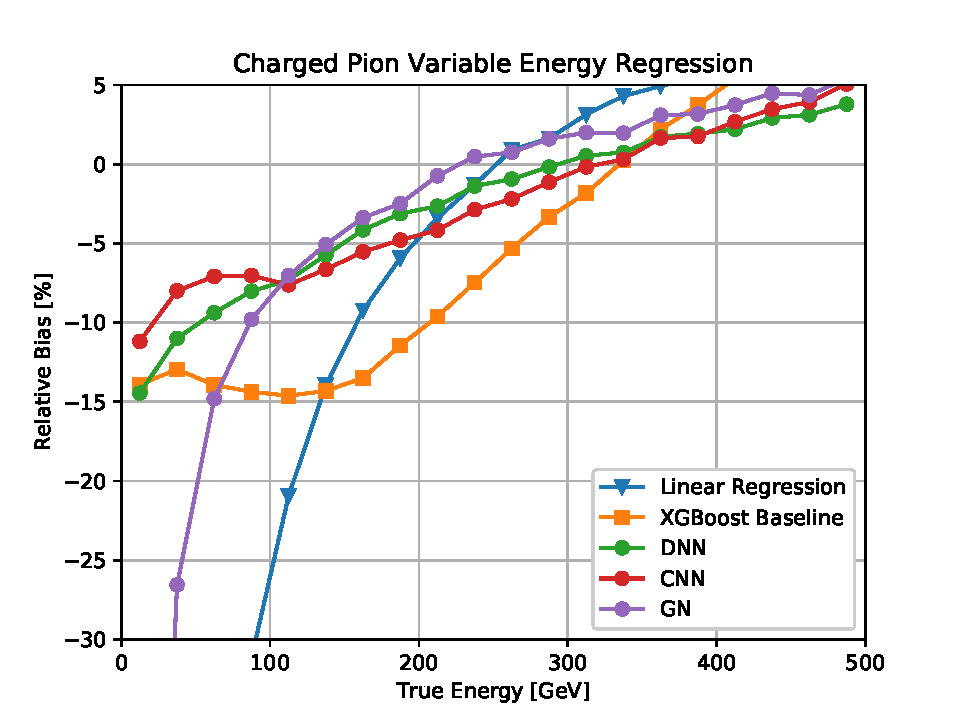
\includegraphics[width=0.38\textwidth]{images/bias_vs_E_ChPi_variable}
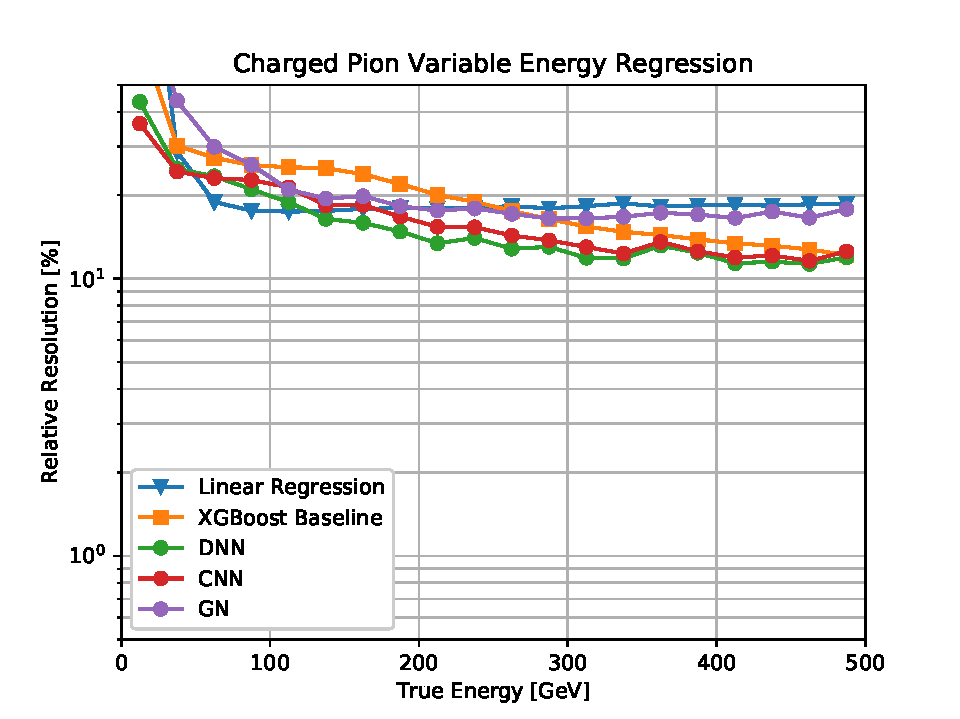
\includegraphics[width=0.38\textwidth]{images/res_vs_E_ChPi_variable}\\
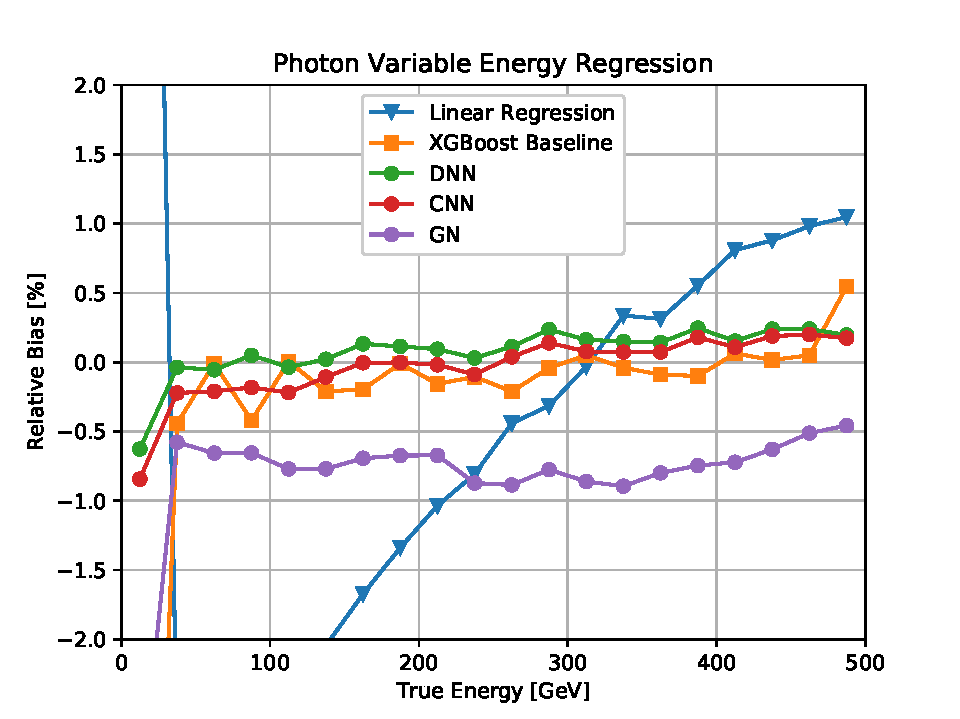
\includegraphics[width=0.38\textwidth]{images/bias_vs_E_Gamma_variable}
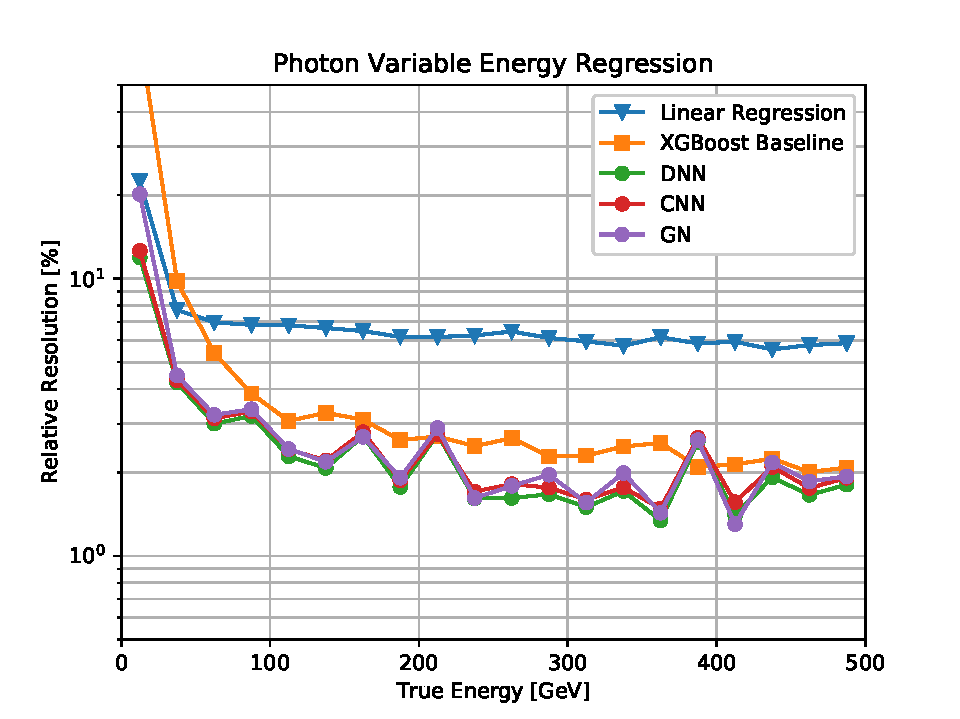
\includegraphics[width=0.38\textwidth]{images/res_vs_E_Gamma_variable}\\
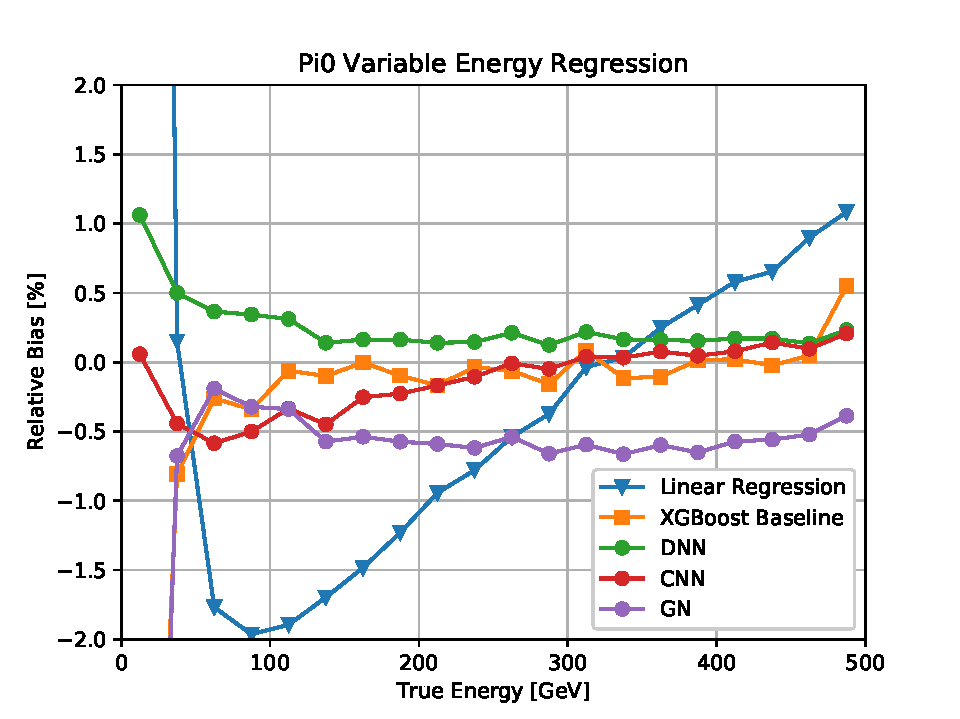
\includegraphics[width=0.38\textwidth]{images/bias_vs_E_Pi0_variable}
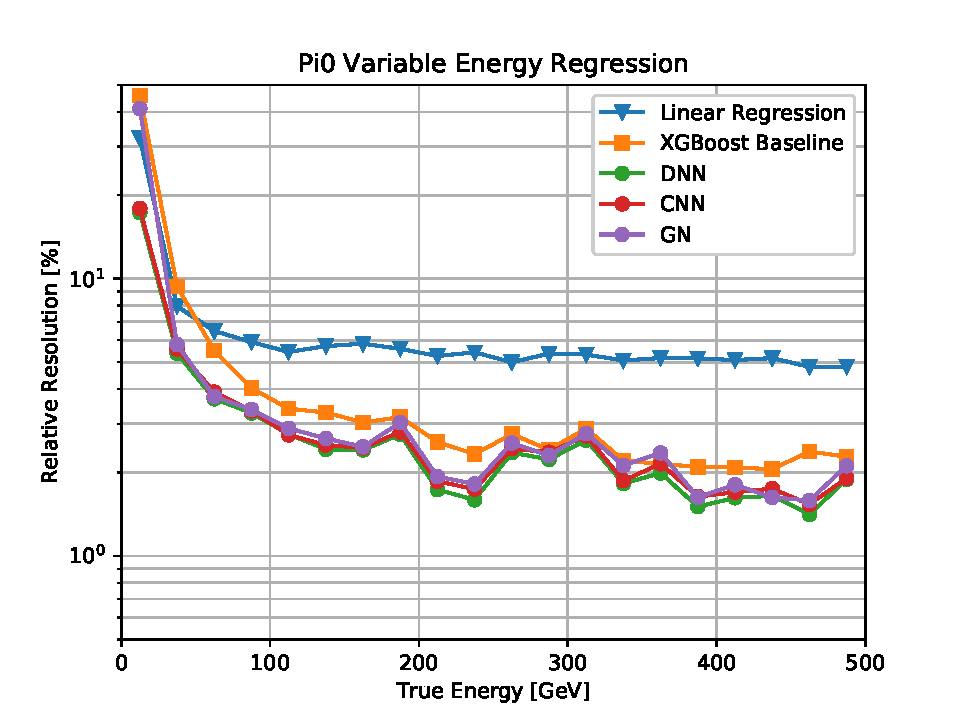
\includegraphics[width=0.38\textwidth]{images/res_vs_E_Pi0_variable}
\caption{Regression bias (top) and resolution (bottom) as a function
  of true energy for energy predictions on the REC dataset with
  variable-angle incident angle. From top to bottom: electrons,
  charged pions, photons, and neutral
  pions.\label{fig:reg_dnn_vs_cnn_variable}}
\end{figure*}

Since the energy regression problem is not as complex as the classification problem, the three architectures (DNN, CNN, GN) perform fairly similarly, with the exception of the GN performance on \chpi, which is a bit worse.
%(and possibly slightly over-trained). 
The performance is overall worse for \chpi, both with the networks and with the benchmark baselines (linear regression and XGBoost).

A closer look at the performance boost given by each network can be obtained examining the case of particles entering the calorimeter inner surface at $90^{\mathrm o}$, i.e. with $\eta=0$~\footnote{For these additional fixed-angle regression plots, we did not train GoogLeNet architectures.}. In this case, the problem is more constrained and both the networks and the baseline algorithms are able to perform accurately. The results for fixed angle samples are shown in Appendix~\ref{app:regression_fixed_angle}.

We have also tested the result of training on one class of particle and performing regression on another. These results can be seen in Appendix~\ref{app:xtrain_regression}. In addition, we have looked at the effect on energy regression of increasing the ECAL and HCAL window sizes. This can be seen in Appendix~\ref{app:large_window_regression}.

\subsection{Resampling to ATLAS and CMS Geometries}\label{sec:resampling}

In addition to the results presented so far, we show in this section how the end-to-end reconstruction would perform on calorimeters with granularity and geometry similar to those of the ATLAS and CMS calorimeters. Since the REC dataset (see Section~\ref{sec:data}) is generated using the geometry of the proposed LCD detector, it has a much higher granularity than the current-generation ATLAS and CMS detectors. To visualize how our calorimeter data would look with a coarser detector, we linearly extrapolate the contents of each event to a different calorimeter geometry, using a process we have termed "resampling". To keep the resampling procedure simple, we discard the HCAL information and consider only the ECAL 3D array.

\begin{table*}[tbp]
\centering
\caption{Detailed description of the three detector geometries used in this study: the baseline CLIC ECAL detector and the ATLAS and CMS calorimeters.\label{tab:resampling_geometry}}
\begin{tabular}{c|c|ccc|c}
\hline
\multirow{2}{*}{Parameter} & \multirow{2}{*}{\textbf{CLIC}} & \multicolumn{3}{c|}{\textbf{ATLAS}} & \multirow{2}{*}{\textbf{CMS}} \\
            &               & 1st layer & 2nd layer & 3rd layer & \\
\hline
$\Delta \eta$         & 0.003  & 0.025 /8 & 0.025 & 0.5   & 0.0175 \\
$\Delta \phi$         & 0.003  & 0.1      & 0.025 & 0.025 & 0.0175 \\
Radiation Length [cm] & 0.3504 & 14       & 14    & 14    & 0.8903 \\
Moliere radios [cm]   & 0.9327 & 9.043    & 9.043 & 9.043 & 1.959  \\
\hline 
\end{tabular}
\end{table*}

A not-to-scale example of the full procedure is shown in Figure~\ref{fig:resampling}. In this example, we resample the input to a regular square grid with lower granularity than the input data. The operation is simplified in the figure, in order to make the explanation easy to visualize. The actual ATLAS and CMS calorimeter geometries are more complex than a regular array, as described in Table~\ref{tab:resampling_geometry}.

In the resampling process, we first extrapolate each energy value from the grid of CLIC cells to a different geometry. To do so, we scale the content of each CLIC cell to the fraction of overlap area between the CLIC cell and the cell of the target geometry. When computing the overlap fraction, we take into account the fact that different materials have different properties (Moliere radius, interaction length, and radiation length). For instance, CLIC is more fine-grained than CMS or ATLAS detectors, but the Moliere radius of the CLIC ECAL is much smaller than in either of those detectors. This difference determines an offset in the fine binning. Thus, when applying our resampling procedure we normalize the cell size by the detector properties. The Moliere radius is used for $x$ and $y$ re-binning, and radiation length is used for the $z$ direction. At this point we have a good approximation for how the event would look in a calorimeter with the target geometry.

To complete the resampling process, we invert the procedure to go back to our original high-granularity geometry. This last step allows us to keep using the model architectures that we have already optimized. It adds no additional information that would not be present in the low-granularity geometry. This up-sampling also allows us to deal with the irregular geometry of the ATLAS calorimeter by turning it into a neat grid. With no up-sampling, it would not be possible to apply the CNN and GN models.

\begin{figure}[htbp]
    \centering
    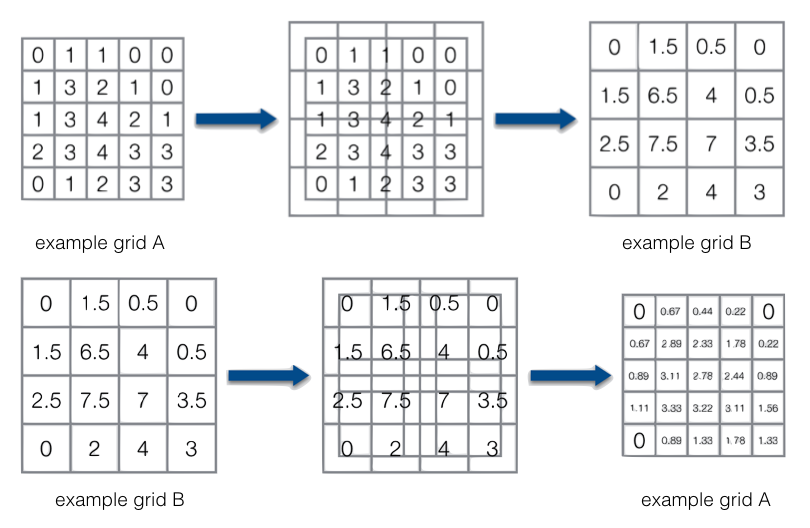
\includegraphics[scale=0.3, clip]{images/resampling.png}
    \caption{Example of the resampling procedure used to emulate CLIC data on a different detector geometry (the example shown here is simply a larger grid). First, we extrapolate hit information from one geometry to another (top). Next, we extrapolate back to the original geometry (bottom). This allows us to emulate the rougher granularity of the second geometry, while keeping data array sizes constant and enabling us to use the models we have already developed for the CLIC dataset. Note that some information is lost at the edges.}
    \label{fig:resampling}
\end{figure}

%\begin{center}
%\begin{tabular}{ l | c c c c c }
% Detector & Cell Size ($\Delta\eta\times\Delta\phi$) & Image Size & Material & $\Chi_0$ [cm] & $R_M$ [cm] \\ 
%\hline
%CLIC          & $0.003\times0.003$     & $25\times25\times25$ & tungsten & 0.35 & 0.92       \\
%CMS           & $0.0175\times0.0175$   & $5\times5\times1$    & lead tungstate & 0.89 & 1.96 \\  
%ATLAS layer 1 & $0.003\times0.1$       & & & & \\
%\caption{Calorimeter properties for the three detector geometries considered. UPDATE FORMAT TO FIT IN ONE COLUMN AND ADD ATLAS 3 LAYERS}
%\end{tabular}
%\end{center}

The resampling procedure comes with a substantial simplification of the underlying physics process. First of all, the information at the edge of the grid is imperfectly translated during the resampling process, leading to worse performance than what could theoretically be achieved in the actual CMS and ATLAS detectors. Also, this simple geometrical rescaling doesn't capture many other detector characteristics. For example, the CMS ECAL detector has no depth information, but being homogeneous it provides a very precise energy measurement. Our resampling method only captures geometric effects, and would not be able to model the improvement in energy resolution. Furthermore, we are unable to include second-order effects such as gaps in the detector geometries. Despite these limitations, one can still extract useful information from the resampled datasets, comparing the classification and regression performances of the end-to-end models defined in Sections~\ref{sec:classification} and~\ref{sec:regression} on different detector geometries.

Comparisons of classification ROC curves between network architectures and our BDT baseline are shown in Figure~\ref{fig:class_ROC_ATLAS_CMS} for ATLAS-like and CMS-like geometries. Here we can see that the previously observed performance ranking still holds true. The GN
model performs best, followed by the CNN, then the DNN. All three networks outperform the BDT baseline. The effect is less pronounced after the CMS-like resampling, due to the low granularity and the single detector layer in the z direction.

\begin{figure}[htbp]
    \centering
    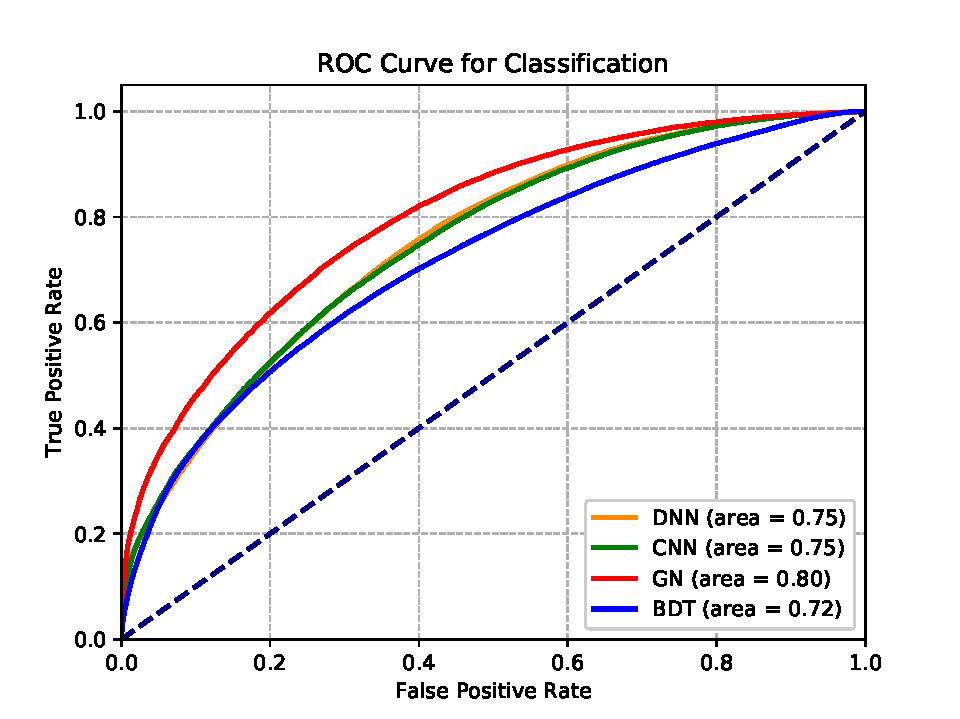
\includegraphics[scale=0.5, clip]{images/classification_ROC_ATLAS}
    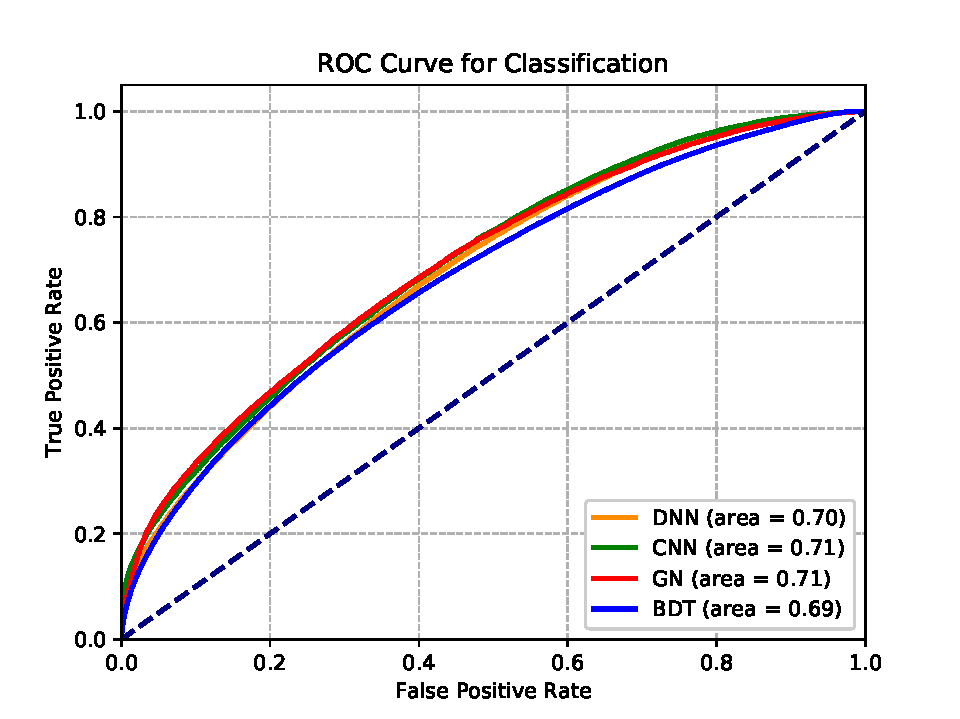
\includegraphics[scale=0.5, clip]{images/classification_ROC_CMS}
    \caption{ROC curve comparisons for variable-angle $\gamma$/$\pi^0$ classification on data resampled to ATLAS-like (top) and CMS-like (bottom) geometries.}
    \label{fig:class_ROC_ATLAS_CMS}
\end{figure}

Regression results are shown in Figure~\ref{fig:reg_resampled_gamma_ATLAS_CMS} and~\ref{fig:reg_resampled_pi0_ATLAS_CMS}, for photons and neutral pions (we did not train electrons or charged pions for this comparison). Here we have included the regression baselines, DNN networks, and CNN networks, but not GN (which we did not train on resampled data). The results obtained for the ATLAS-like resampling match those on the REC dataset, with DNN and CNN matching the BDT outcome in terms of bias and surpassing it in resolution. With the CMS-like resampling the neural networks match but do not improves over the BDT energy regression resolution. Once again, this is due to the low spatial resolution in the CMS-like geometry, especially due to the lack of $z$ segmentation. We are unable to model the improved energy resolution from the actual CMS detector, so these energy regression results are based on geometry only.

\begin{figure*}[htbp]
\centering
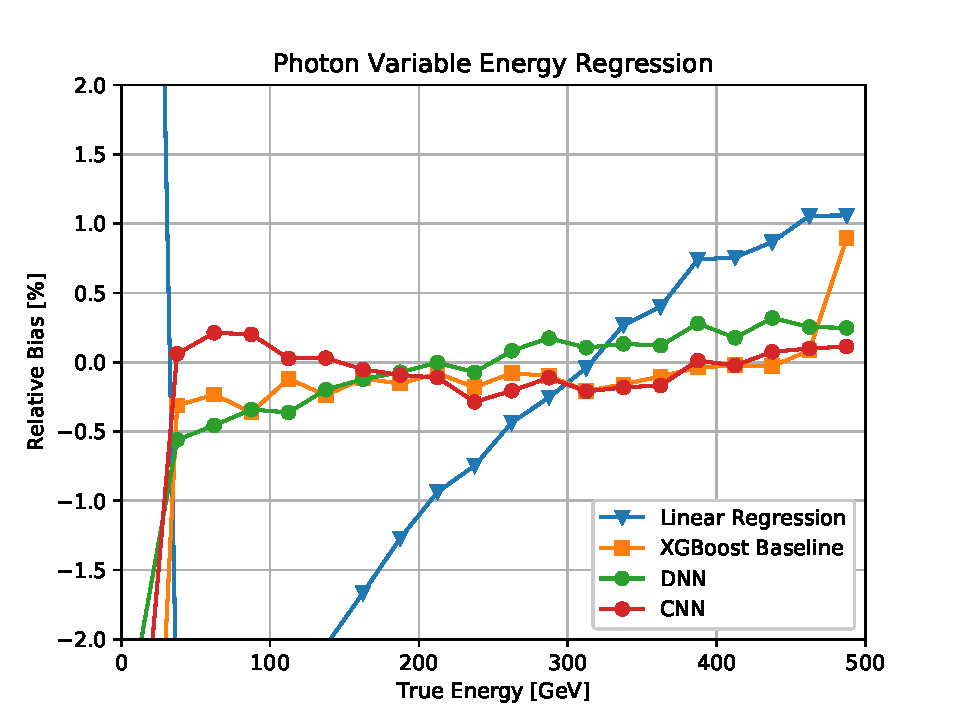
\includegraphics[width=0.38\textwidth]{images/bias_vs_E_Gamma_variable_ATLAS}
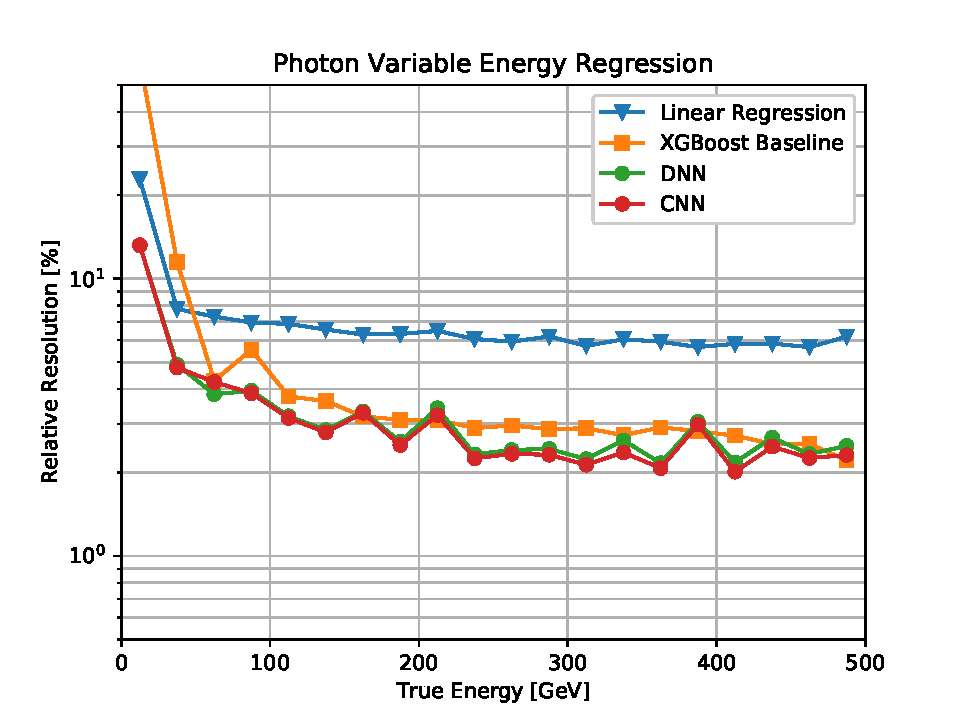
\includegraphics[width=0.38\textwidth]{images/res_vs_E_Gamma_variable_ATLAS} \\
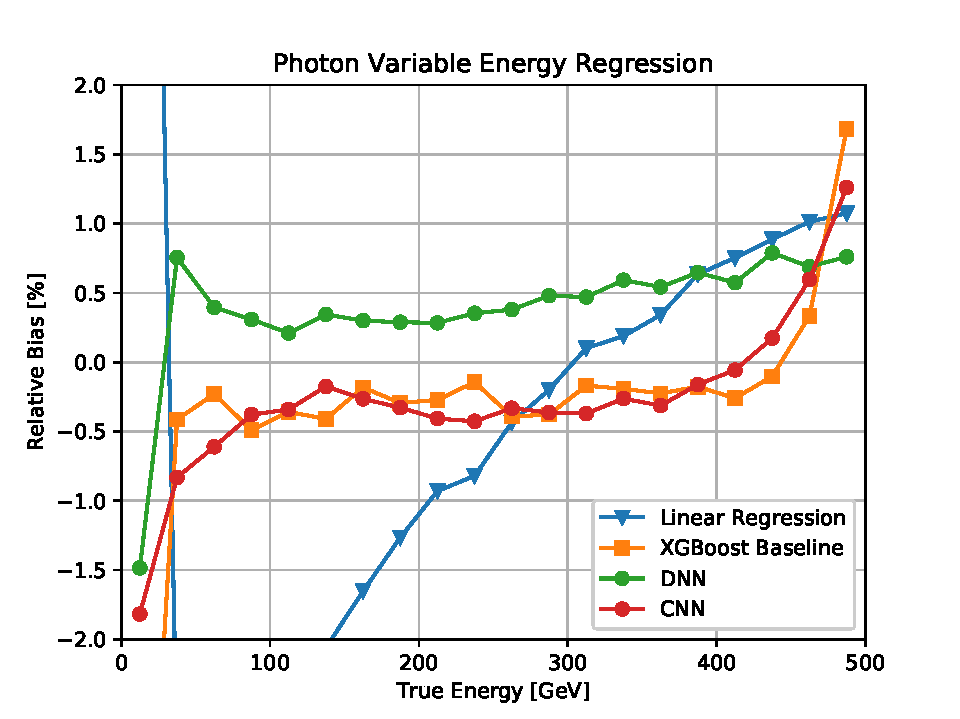
\includegraphics[width=0.38\textwidth]{images/bias_vs_E_Gamma_variable_CMS}
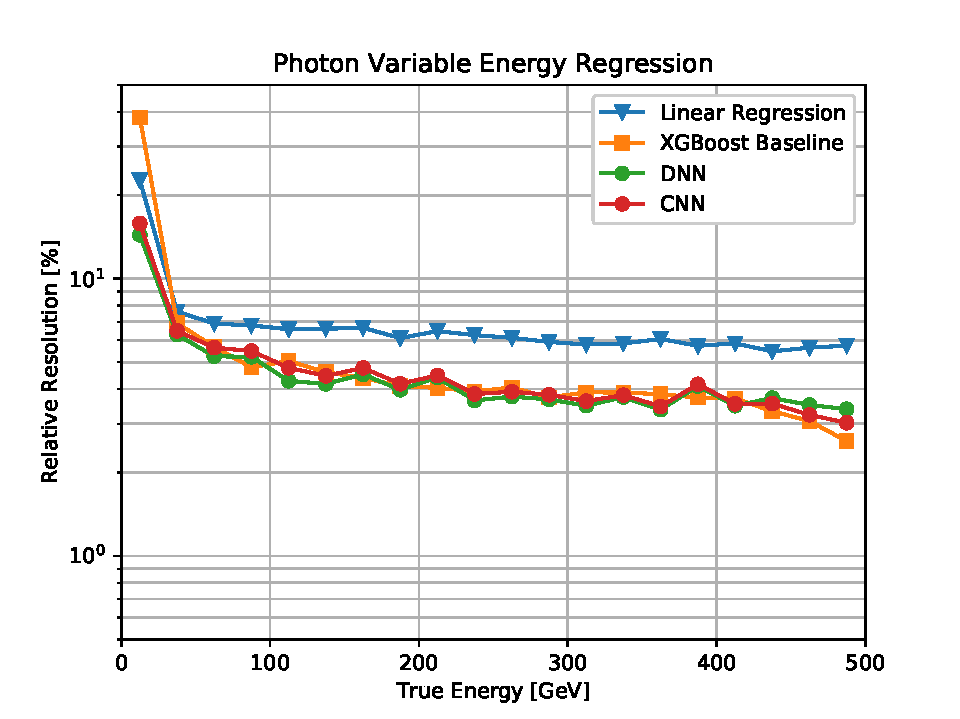
\includegraphics[width=0.38\textwidth]{images/res_vs_E_Gamma_variable_CMS}
\caption{Bias (left) and resolution (right) as a function of true energy for energy predictions for photons, on variable-angle samples resampled to ATLAS-like (top) and CMS-like (bottom) geometries.\label{fig:reg_resampled_gamma_ATLAS_CMS}}
\end{figure*}

\begin{figure*}[htbp]
\centering
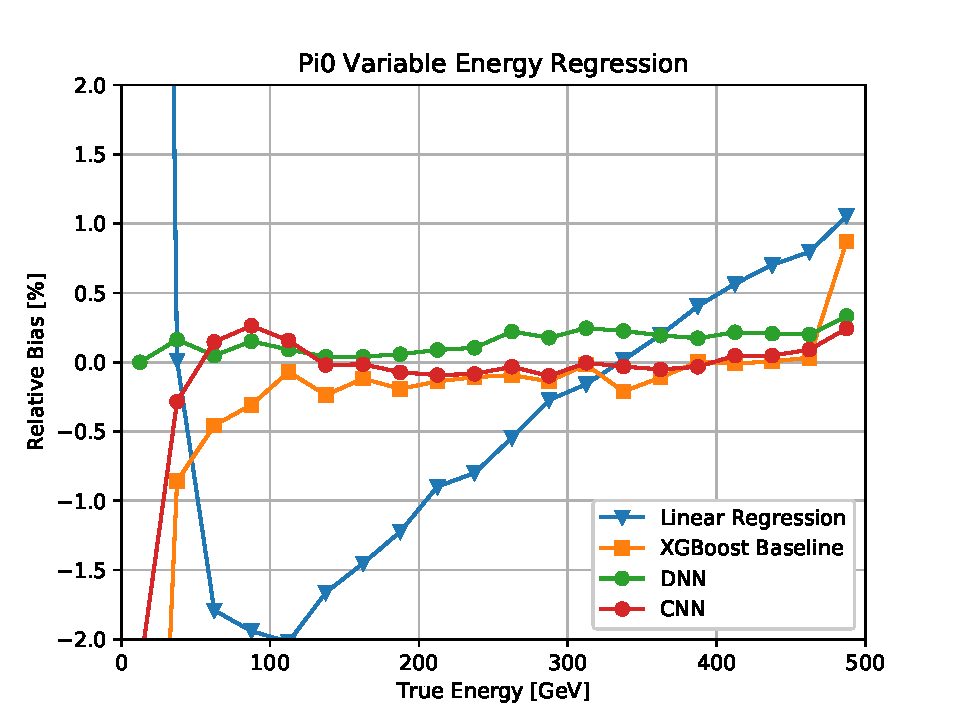
\includegraphics[width=0.38\textwidth]{images/bias_vs_E_Pi0_variable_ATLAS}
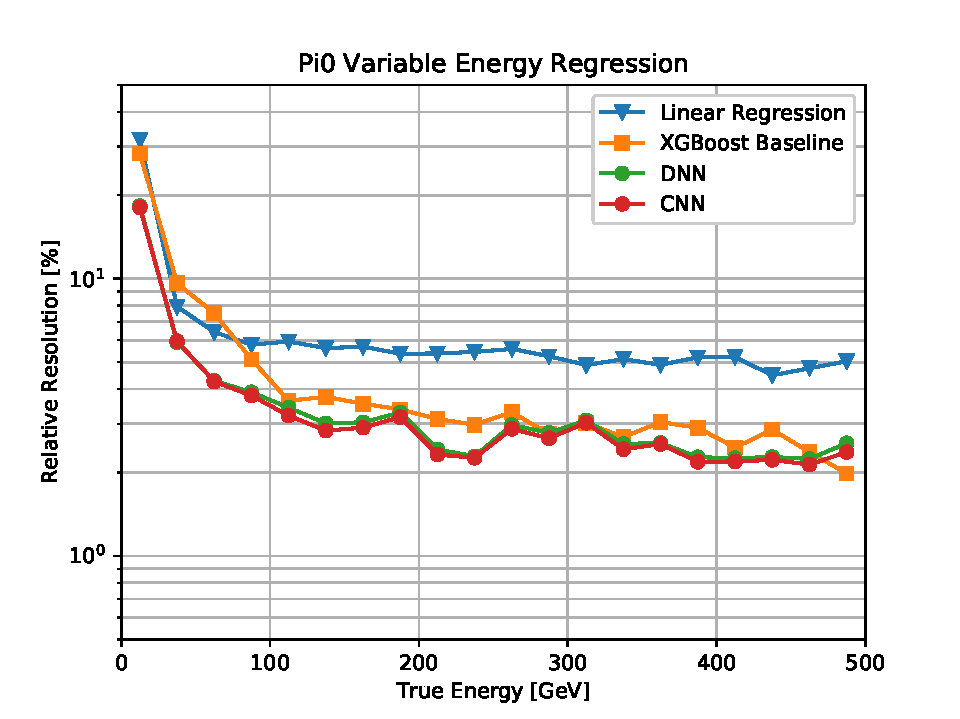
\includegraphics[width=0.38\textwidth]{images/res_vs_E_Pi0_variable_ATLAS} \\
\includegraphics[width=0.38\textwidth]{images/bias_vs_E_Pi0_variable_CMS}
\includegraphics[width=0.38\textwidth]{images/res_vs_E_Pi0_variable_CMS}
\caption{Bias (left) and resolution (right) as a function of true energy for energy predictions for \pizero, on variable-angle samples resampled to  ATLAS-like (top) and CMS-like (bottom) geometries.\label{fig:reg_resampled_pi0_ATLAS_CMS}}
\end{figure*}

\section{GAN}

\section{Generative Model}\label{sec:GAN}

Generative Adversarial Networks are composed of two networks, a discriminator and a generator. Our model, 3DGAN, implements an architecture inspired by the auxiliary classifier GAN~\cite{acgan}. The generator takes as input a specific particle type, flight direction, and energy, and generates the 3D image of an energy deposit using an auxiliary input vector of random quantities (latent vector). 
The output has the same format as the 3D array of ECAL hits in the GEN sample (see Section~\ref{sec:data}). The discriminator network receives as input an ECAL 3D array and classifies it as {\it real} (coming from the GEANT4-generated GEN dataset) or {\it fake} (produced by the generator).

 Our initial 3DGAN prototype~\cite{NIPS} successfully simulated detector outputs for electrons which were orthogonally incident to the calorimeter surface. In addition, the discriminator performed an auxiliary regression task on the input particle energy. This task was used to cross check the quality of the generation process. 
 
 In this study, we consider a more complex dataset, e.g., due to the variable incident angle of the incoming electron on the inner ECAL surface. To monitor this additional complexity, we add additional components to the loss function, related to the regression of the particle direction and the pixel intensity distribution (energy deposition in cells). This will be described in more detail below.

Before training our GAN, we pre-processed the GEN dataset by replacing each cell energy content $E$ with $E^\alpha$, where $\alpha<1$ is a fixed hyperparameter. This pre-processing compensates for the large energy range (about 7 orders of magnitude) covered by individual cell energies, and mitigates some performance degradation we previously observed at low energies. After testing for different values of $\alpha$, we observed optimal performance for $\alpha=0.85$.

\begin{figure*}[htbp]
\centering
    \includegraphics[scale=0.65, trim={0cm 6cm 3.5cm 1.8cm}]{images/gan_model_alt_upsampling.pdf}
    \caption{3DGAN generator and discriminator network architectures}
    \label{fig:GAN_arch}
\end{figure*}

\subsection{GAN Architecture}
\label{sec:GANarch}

The 3DGAN architecture is based on 3-dimensional convolutional layers, as shown in Figure~\ref{fig:GAN_arch}. The generator takes as input a vector with a desired particle energy and angle, and concatenates a latent vector of 254 normally distributed random numbers. This goes through a set of alternating upsampling and convolutional layers. The first convolution layer has $64$ filters with $6 \times 6 \times 8$ kernels. The next two convolutional layers have $6$ filters of $5 \times 8 \times 8$ and $3 \times 5 \times 8$ kernels, respectively. The last convolutional layer has a single filter with a $2 \times 2 \times 2$ kernel. The first three layers are activated by leaky ReLU functions, while ReLU functions are used for the last layer. Batch normalization and upscaling layers were added after the first and second convolutional layers.

The discriminator takes as input a $51  \times 51  \times 25$ array and consists of four 3D convolutional layers. The first layer has $16$ filters with $5 \times 6 \times 6$ kernels. The second, third, and fourth convolutional layers each have $8$ filters with $5 \times 6 \times 6$ kernels. There are leaky ReLU activation functions in each convolutional layer. Batch normalization and dropout layers are added after the second, third, and fourth convolutional layers. The output of the final convolution layer is flattened and connected to two output nodes: a classification node, activated by a sigmoid and returning the probability of a given input to be true or fake; and a regression node, activated by a linear function and returning the input particle energy.
The 3DGAN model is implemented in KERAS~\cite{keras} and Tensorflow~\cite{tensorflow2015-whitepaper}. 

\subsection{Training and Results}
The 3DGAN loss function
\begin{equation}
   L_{Tot}  = W_{G}L_{G} + W_{P}L_{P} + W_{A}L_{A} + W_{E}L_{E} + W_{B}L_{B} 
\label{eq:loss}
\end{equation}
is built as a weighted sum of several terms: a binary cross entropy ($L_{G}$) function of the real/fake probability returned by the discriminator, mean absolute percentage error terms (MAPE) related to the regression of the primary-particle energy ($L_{P}$) , the total deposited energy ($L_{E}$) and the binned pixel intensity distribution ($L_{B}$), and a mean absolute error (MAE) for the incident angles measurement ($L_{A}$). The binary cross entropy term, percentage errors and absolute error are weighted by $3.0$, $0.1$ and $25$ respectively. The weights $W$ are tuned to balance the relative importance of each contribution. The predicted energy and incident angle provide a feedback on the conditioning of the image. The binned pixel intensity distribution loss compares the counts in different bins of pixel intensities. 

The model training is done using the RMSprop \cite{rmsProp} optimiser. We alternately train the discriminator on a batch of real images and a batch of generated images, applying label switching. We then train the generator while freezing the discriminator weights.

Figure~\ref{fig:GEANT4_events} shows a few events from the GEN data set. The events were selected to cover both ends of the primary-particle energy and angle spectrum. Figure~\ref{fig:GAN_events} presents the corresponding generated events with the same primary particle energy and angle as the GEN events in Figure~\ref{fig:GEANT4_events}. Initial visual inspection shows no obvious difference between the original and GAN generated images. A detailed validation based on several energy-shape related features confirms these results. We discuss a few examples below.

\begin{figure}[htbp]
    \includegraphics[width=0.48\textwidth]{images/GAN_g4_events.pdf}
    \caption{GEN sample: electrons with different primary particle energies and angles.}
    \label{fig:GEANT4_events}
\end{figure}

\begin{figure}[htbp]
    \includegraphics[width=0.48\textwidth]{images/GAN_gan_events.pdf}
    \caption{GAN generated electrons with primary energies and angles corresponding to the electrons showed in Figure~\ref{fig:GEANT4_events}.}
    \label{fig:GAN_events}
\end{figure}

The top row in Figure~\ref{fig:GAN_features1} shows the ratio between the total energy deposited in the calorimeter and the primary particle energy as a function of the primary particle energy (we refer to it as "sampling fraction") for different angle values. 3DGAN can nicely reproduce the expected behaviour over the whole energy spectrum. The second row in Figure~\ref{fig:GAN_features1} shows the number of hits above a $3 \times 10^{-4}$ MeV threshold. Figure~\ref{fig:GAN_features1} also shows the x, y, z "energy shapes", i.e. the amount of energy deposited along different axes (x and y on the transverse plane and z along the calorimeter depth). The agreement is very good, and in particular 3DGAN is able to mimic the way the energy distributions changes with incident angle. 
Figure~\ref{fig:GAN_features2} shows some additional features aimed at defining the shape of the deposited energy distribution. In particular the second moments along the x,y and z axes are shown on the first column, measuring the width of the deposited energy distribution along those axes. The second column shows the way the energy is deposited along the depth of the calorimeter, by splitting the calorimeter in three parts along the longitudinal direction and measuring the ratios between the energy deposited in each third  and the total deposited energy. Finally, the third column in Figure~\ref{fig:GAN_features2} highlights the tails of the "energy shapes". It can be seen that, while the core of the distribution is perfectly described by 3DGAN, the network tends to overestimate the amount of energy deposited at the edges of the volume. It should be noted however that energy depositions in those cells are very sparse. 
\iffalse
\begin{figure}
    \centering
    \includegraphics[scale=0.3]{images/GAN_feature_ECAL_E.png}
    \includegraphics[scale=0.3]{images/GAN_feature_ECAL_nHits.png}
    \includegraphics[scale=0.3]{images/GAN_feature_ECAL_ratioFirstLayerToSecondLayerE.png}
    \includegraphics[scale=0.3]{images/GAN_feature_ECAL_ratioFirstLayerToTotalE.png}
    \includegraphics[scale=0.3]{images/GAN_feature_ECALmomentX1.png}
    \includegraphics[scale=0.3]{images/GAN_feature_ECALmomentX2.png}
    \includegraphics[scale=0.3]{images/GAN_feature_ECALmomentX3.png}
    \includegraphics[scale=0.3]{images/GAN_feature_ECALmomentY1.png}
    \includegraphics[scale=0.3]{images/GAN_feature_ECALmomentZ1.png}
    \includegraphics[scale=0.3]{images/GAN_feature_R9.png}
    \caption{GAN vs. GEANT comparisons for various features. {\bf theta should be $\theta$.}
    \label{fig:GAN_features}}
\end{figure}
\fi
\begin{figure}
    \centering
    \includegraphics[width=0.48\textwidth]{images/features_1.pdf}
    \caption{GEANT4 vs. GAN comparison for sampling fraction, number
      of hits and shower shapes along x,y,z axis for different angle
      bins with 100-200 GeV primary particle energies.
      \label{fig:GAN_features1}}
\end{figure}

\begin{figure}
    \centering
    \includegraphics[width=0.48\textwidth]{images/features_2.pdf}
    \caption{GEANT4 vs. GAN comparison for shower width (second
      moment) in x,y,z, ratio of energy deposited in parts along
      direction of particle traversal to total energy and shower
      shapes along x,y,z axis in log scale for 100-200 GeV primary
      particle energies and 60-120 degrees $\theta$.
      \label{fig:GAN_features2}}
\end{figure}

The 3DGAN training runs in around $1.5$ hours per epoch on a single NVIDIA GeForce GTX 1080 card for $60$ epochs. The simulation  time  on a Intel  Xeon 8180  is about $13$ ms/particle  and it goes down to about $4$ ms/particle on a NVIDIA  GeForce  GTX  1080. For  comparison  GEANT4  simulation takes  about $17$ seconds  per  particle on  a  Intel  Xeon  8180 (currently  it  is  not  possible  to  run a full  GEANT4-based  simulation  on  GPUs). Thus our GAN represents a potential simulation speedup of over 4,000 times for this specific aspect of the event simulation.

When given as input to a particle regression and reconstruction model (see section~\ref{sec:reco}), this dataset produces the same output as the original GEANT4 sample, as described in Appendix~\ref{appendix:RECO_on_GAN}.

\section{Conclusion}

This paper shows how deep learning techniques could outperform traditional and resource-consuming techniques in  tasks typical of physics experiments at particle colliders, such as particle shower simulation and reconstruction in a calorimeter.
We consider several model architectures, notably 3D convolutional neural networks, and we show competitive performance, matched to short execution time. In addition, this strategy comes with a GPU-friendly computing solution and would fit the current trends in particle physics towards heterogeneous computing platforms. 

We confirm findings from previous studies of this kind. On the other hand, we do so utilizing a fully accurate detector simulation, based on a complete GEANT4 simulation of a full particle detector, including several detector components, magnetic field, etc. In addition, we design the network so that different tasks are performed by a single architecture, optimized through an hyperparameter scan. 

We look forward to the development of similar solutions for current and future particle detectors, for which this kind of end-to-end solution could be extremely helpful. 

\part{Identifying  Heavy-Flavor  Leptons  Using  Recurrent  Neural Nets}
\chapter{Identifying Heavy-Flavor Leptons Using Recurrent Neural Nets}

\section{What Are We Doing?}

\subsection{The Problem}

\subsection{The Tools}

\subsection{The People}

\section{Data Preparation}

\section{Neural Architectures}

\section{Classification}

\section{Conclusion}

\part{Another Search for Supersymmetry}
%%%%%%%%%%%%%%%%%%%%%%%%%%%%%%%%%%%%%%%%%%%%%%%%%%%%%%%%%%%

Previously, I participated in a search for SUSY, targeting the events shown in Figure~\ref{SUSY_2l2j}. In these events, an initial gluon decays into a $\tilde{\chi}^0_2$ (second-lightest neutralino) and two quarks. The $\tilde{\chi}^0_2$ further decays into $\tilde{\chi}^0_1$ (lightest neutralino) via either a Z boson decay or an intermediate slepton decay. The Z may be either on or off shell. To target these decays, we looked for events with final states containing a same-flavour opposite-sign lepton (electron or muon) pair, two or more jets, and large missing transverse momentum ($E_T^{miss}$). To differentiate between the different models (on-shell Z, off-shell Z, and slepton decay), we looked at the final dilepton mass distribution, as seen in Figure~\ref{mll}. These searches used $\sqrt{s}$ = 13 TeV collision data with an integrated luminosity of $14.7 fb^{-1}$, gathered by the ATLAS detector during 2015 and 2016.

\begin{figure}[t]
    \centering
    \includegraphics[width=0.7\linewidth]{images/SUSY_2l2j.png}
    \caption{SUSY models involving final states with two leptons, two jets, and large transverse missing energy. Note that though these diagrams show two gluino decay branches, the final state we searched for only required one.}
    \label{SUSY_2l2j}
\end{figure}

\begin{figure}[t]
    \centering
    \includegraphics[width=0.5\linewidth]{images/mll.png}
    \caption{Different dilepton mass ($m_{ll}$) distributions. On-shell Z bosons have an $m_{ll}$ peak around the Z mass at 91 GeV, but off-shell Z's would see a sharp cutoff in the $m_{ll}$ distribution at an energy equal to $m_{\tilde{\chi}^0_2} - m_{\tilde{\chi}^0_1}$. Events which went through the slepton decay process would see an entirely different $m_{ll}$ distribution shape.}
    \label{mll}
    
	\centering
    \includegraphics[width=0.45\linewidth]{images/slepton_signal_regions.png}
    \includegraphics[width=0.45\linewidth]{images/Z_signal_regions.png}
    \caption{Signal regions chosen to maximize signal-over-background ratios given various sparticle masses. The signal regions on the left are for slepton and off-shell Z models, and correspond to low, medium, and high values of $m_{\tilde{\chi}^0_2} - m_{\tilde{\chi}^0_1}$. The signal region on the right is for the on-shell Z model. $H_T$ refers to the total transverse momentum of jets.}
    \label{signal_regions}
\end{figure}

When selecting objects for this analysis, we decided to use signal leptons with transverse momentum ($p_T$) above 25 GeV, and jets with $p_T$ above 30 GeV. For the purposes of performing jet overlap removal and calculating $E_T^{miss}$, we also allowed baseline leptons above 10 GeV and baseline jets above 20 GeV. In the interest of keeping this paper at a reasonable length, the complete set of object selection and triggering criteria will not be included, but can be found in the complete SUSY analysis paper at \cite{SUSY_2l2j}.

As with most high-energy physics searches, there were a variety of standard-model processes which mimicked the final state we were looking for. Of these, the $t\bar{t}$ process was the largest, followed by diboson (WZ/ZZ) processes. Events with a single Z and two or more jets from initial-state radiation could also mimic our signal, provided that mismeasurement of the jet momentum resulted in a large $E_T^{miss}$ for the event. Events from single-top-quark processes and from lepton misidentification also contributed to the background. To accurately model these backgrounds, we used flavor-symmetry, Z/$\gamma^*$, Monte Carlo, and fake estimation methods, all of which will be described below.

As we had several unknown masses in our models, we needed to find multiple signal regions which could optimize the signal-to-background ratio for a variety of different $\tilde{\chi}^0_1$, $\tilde{\chi}^0_2$, and $\tilde{g}$ masses. In Figure~\ref{signal_regions}, we show the four signal regions we chose, along with their associated validation and control regions, which were used to implement and test various background-rejection methods.

\subsection*{Flavor Symmetry}

Flavor symmetry (FS) was an important background rejection method, and removed contributions from processes such as $Z\rightarrow\tau\tau$, $t\tilde{t}$, WW, and tW. Unlike our signal models, which produced only pairs of same-flavor leptons, these processes could produce same-flavor and opposite-flavor lepton pairs with equal probability. The basic idea was to take the opposite-flavor $e\mu$ events from data in each signal region, and to use them to estimate the number of same-flavor events from FS sources in each of those regions. Due to differences in detection and triggering efficiencies for electrons and muons, we had to apply the scaling factor shown in the following equation, where $\epsilon_{e/\mu}$ was the offline selection efficiency for each lepton and $\epsilon_{e\mu/ee}^{trigger}$ was the dilepton trigger efficiency for each channel. The equation for the $\mu\mu$ channel followed the same logic.

\begin{gather}
%n_{ee}^{measured} = n_{ee}^{truth}\epsilon_e^2\epsilon_{ee}^{trigger} \\
%n_{e\mu}^{measured} = n_{e\mu}^{truth}\epsilon_e\epsilon_{\mu}\epsilon_{e\mu}^{trigger} \\
n_{ee}^{measured} = \frac{1}{2}\frac{\epsilon_e}{\epsilon_{\mu}}\frac{\epsilon_{ee}^{trigger}}{\epsilon_{e\mu}^{trigger}}n_{e\mu}^{measured}
\end{gather}

\subsection*{Z/$\gamma^*$ + Jets}

Another important background was single-Z events with two additional jets from initial state radiation. There was no real missing energy in these events, but they could appear to have $E_T^{miss}$ due to mismeasurement of jet momentum. Jets were difficult to model accurately in Monte Carlo simulation due to the complexity of hadronic showering, so to estimate Z + jets, we used a data-driven method where we selected for a similar background ($\gamma$ + jets), and applied reweighting and momentum smearing. Since in this case both $\gamma$ and $Z\rightarrow ll$ were well-measured particles recoiling against two jets, the kinematics of both processes were very similar. One difference came from the fact that $\gamma$ is massless, which caused its $p_T$ distribution to be different from that of Z. We had to correct for this by reweighting $\gamma$ events in bins of $p_T$. Photon $p_T$ also had to be smeared to match the resolution of muon $p_T$ in the $Z\rightarrow\mu\mu$ channel.

%There were also differences in resolution, since photons and electrons were measured quite accurately, but muons had worse resolution, especially at high $p_T$. Thus, to account for the fact that $Z\rightarrow\mu\mu$ events had worse resolution, photon $p_T$ had to be smeared to match the resolution of Z $p_T$ in the $\mu\mu$ channel.

%\begin{figure}[t]
%    \centering
%    \includegraphics[width=0.8\linewidth]{images/gamma_jets.png}
%    \caption{We selected events in data with $\gamma$ + jets and no leptons (left), and used them to estimate the background contribution from Z + jets (right).}
%    \label{gamma_jets}
%\end{figure}

\subsection*{Fake Leptons}

Another contribution to background came from events where one or more non-leptonic objects were incorrectly identified as leptons. Semileptonic $t\bar{t}$, W + jets, and single top events were included in this category. We estimated the number of fake leptons in each region using a matrix method described in detail in \cite{fake_method}. The general idea was that in each signal region, we would apply both loose and tight lepton selections. We labeled the number of baseline (loose) leptons which passed the signal (tight) cut as $N_{pass}$, and called the ones which failed $N_{fail}$. Given two further numbers, $\epsilon^{real}$ and $\epsilon^{fake}$ (fractions which pass the signal cut), we could then estimate the number of fake signal leptons using the following equation. $\epsilon^{real}$ and $\epsilon^{fake}$ were calculated via a tag-and-probe approach. Expanding this method to a dilepton system (where either or both leptons could be fake) required only that we extend this logic to a 4x4 matrix.

\begin{equation}
N_{pass}^{fake} = \frac{N_{fail}-(1/\epsilon^{real}-1)\times N_{pass}}{1/\epsilon^{fake}-1/\epsilon^{real}}.
\end{equation}

%Using this equation required that we obtain good estimates for $\epsilon^{real}$ and $\epsilon^{fake}$. We could find $\epsilon^{real}$ by looking in a signal region which selected for a high concentration of likely $Z\rightarrow ll$ events, and by performing a tag-and-probe method with the leading lepton as the tag. We estimated $\epsilon^{fake}$ in a similar way, by looking in a region with high likelihood of fake leptons (requiring exactly two same-sign leptons), and using the lower-$p_T$ lepton to calculate $\epsilon^{fake}$. For the fake-lepton region, we made sure to disregard same-sign dilepton events which came about as a result of prompt lepton production. These processes were simulated in Monte Carlo, and subtracted from the data. Expanding this method to a dilepton system (where either or both leptons could be fake) required only that we extend this logic to a 4x4 matrix. Fake lepton rates were calculated in $p_T$ bins for each region.

\subsection*{Monte Carlo}

Finally, we come to the section that I was responsible for, the Monte Carlo simulation of diboson events, mainly $WZ\rightarrow lll\nu$ and $ZZ\rightarrow ll\nu\nu$, as well as the simulation of smaller diboson processes and other rare events such as ttZ, ttW, ttWWW, etc. Modeling for the two major diboson components (which make up about $20-30\%$ of the background in each region) was validated in three regions, VR-WZ, VR-ZZ, and VR-3L. VR-WZ and VR-3L were both intended to validate the WZ process, just in different regions of phase space. VR-ZZ was a four-lepton region meant to validate the $ZZ\rightarrow llll$ process, taking advantage of similarities in the MC simulation process for $ZZ\rightarrow ll\nu\nu$ and $ZZ\rightarrow llll$. These regions were all chosen to be above $90\%$ pure in diboson processes. Data-MC comparisons of $E_T^{miss}$, $H_T$, jet multiplicity, and boson $p_T$ in these regions showed good agreement, demonstrating that there were no difficulties with QCD modeling. Particular attention was paid to MC simulation of jet parameters, and differences between Powheg and Sherpa-generated samples for each region were included in the systematic errors.

The Powheg generator had better jet-modeling properties overall. However, due to the way Powheg produced $ll\nu\nu$ samples, the $WW\rightarrow ll\nu\nu$ and $ZZ\rightarrow ll\nu\nu$ processes could not be separated at the truth level. Since the WW process was already included in the flavor-symmetry method, we had to remove it in order to avoid double-counting. To do this, we estimated the ZZ component in each region by subtracting the DF component of $VV\rightarrow ll\nu\nu$ from the SF component. Since the ZZ process is expected to be much greater than the WW component only in the on-Z $m_{ll}$ region, we calculated systematics for this method by taking the off-Z $m_{ll}$ component of each region and checking the exactness of SF and DF cancellation.

\subsection*{Results}

Results for each signal region are shown in Figure~\ref{results}. The on-Z region shows a significance of $0.47\sigma$, and the largest local significance in any slepton region is $1.7\sigma$. Based on these results, we obtain the exclusion contours in Figure~\ref{exclusion}. In conclusion, this search found only results consistent with the standard model. As seen from the exclusion plots, we have two possible avenues to consider if we wish to extend this search. We can either go towards the higher-mass region, or we could look at the compressed-mass region where mass differences between SUSY particles are very small.

\begin{figure}[t]
    \centering
    \includegraphics[width=0.4\linewidth]{images/slepton_results.png}
    \includegraphics[width=0.45\linewidth]{images/on-Z_results.png}
    \caption{(left) Data-MC comparisons for slepton models. (right) Data-MC comparisons for on-Z model.}
    \label{results}
\end{figure}

\begin{figure}[t]
    \centering
    \includegraphics[width=0.45\linewidth]{images/slepton_exclusion.png}
    \includegraphics[width=0.45\linewidth]{images/on-Z_exclusion.png}
    \caption{(left) Exclusion contours in $m_{\tilde{\chi}_1^0}$, $m_{\tilde{g}}$ space for slepton models where $m_{\tilde{\chi}_2^0} = \frac{1}{2}(m_{\tilde{g}} + m_{\tilde{\chi}_1^0})$. (right) Exclusion contours for on-Z models where $m_{\tilde{\chi}_2^0} = m_{\tilde{\chi}_1^0} + 100$ GeV.}
    \label{exclusion}
\end{figure}

There are good theoretical reasons to look at the compressed-mass region. As mentioned previously, the SUSY gauge particles combine into mass eigenstates called the neutralinos ($\tilde{\chi}^0_{1,2,3,4}$) and charginos ($\tilde{\chi}^\pm_{1,2}$). Together, all these particles are collectively known as electroweakinos. The neutralinos are formed from the photino, zino, and neutral Higgsinos, where the photino and zino are themselves mixtures of the bino and neutral wino. The charginos are formed from the charged winos and charged Higgsinos. If we consider a situation (motivated by naturalness arguments) where the Higgsino mass is close to the weak scale, but the masses of the bino and wino are much higher \cite{Higgsino}, then the lightest electroweakinos ($\tilde{\chi}^0_1, \tilde{\chi}^0_2, \tilde{\chi}^\pm_1$) would be dominated by Higgsino contributions, and in this case their masses would be separated in the range of hundreds of MeV to tens of GeV, putting the model outside the exclusion limits of our previous search.

A previous search using the Higgsino model excluded (with $95\%$ confidence) next-to-lightest neutralino masses of up to 130 GeV, and down to mass splittings of 3 GeV \cite{Higgsino}. Since this model involves very soft (low-pT) leptons, we can improve the sensitivity of the search if we created a more accurate method of identifying and measuring particles at low energy. One way we can improve upon traditional particle identification techniques is to make use of new methods in machine learning and image recognition on raw detector data. An approach for developing such a tool will be described in the following sections. After building the tool, we aim to enhance the search using ATLAS data gathered through the end of LHC Run II (about 100 $fb^{-1}$).


\appendix
%\input{Appendices/blah.tex}

\backmatter
%\bibliography{thesisbib}

\end{document}